% Options for packages loaded elsewhere
\PassOptionsToPackage{unicode}{hyperref}
\PassOptionsToPackage{hyphens}{url}
%
\documentclass[
  12pt,
]{article}
\usepackage{amsmath,amssymb}
\usepackage{lmodern}
\usepackage{iftex}
\ifPDFTeX
  \usepackage[T1]{fontenc}
  \usepackage[utf8]{inputenc}
  \usepackage{textcomp} % provide euro and other symbols
\else % if luatex or xetex
  \usepackage{unicode-math}
  \defaultfontfeatures{Scale=MatchLowercase}
  \defaultfontfeatures[\rmfamily]{Ligatures=TeX,Scale=1}
\fi
% Use upquote if available, for straight quotes in verbatim environments
\IfFileExists{upquote.sty}{\usepackage{upquote}}{}
\IfFileExists{microtype.sty}{% use microtype if available
  \usepackage[]{microtype}
  \UseMicrotypeSet[protrusion]{basicmath} % disable protrusion for tt fonts
}{}
\makeatletter
\@ifundefined{KOMAClassName}{% if non-KOMA class
  \IfFileExists{parskip.sty}{%
    \usepackage{parskip}
  }{% else
    \setlength{\parindent}{0pt}
    \setlength{\parskip}{6pt plus 2pt minus 1pt}}
}{% if KOMA class
  \KOMAoptions{parskip=half}}
\makeatother
\usepackage{xcolor}
\IfFileExists{xurl.sty}{\usepackage{xurl}}{} % add URL line breaks if available
\IfFileExists{bookmark.sty}{\usepackage{bookmark}}{\usepackage{hyperref}}
\hypersetup{
  pdftitle={R 입문 기말고사},
  pdfauthor={김남윤(202121204)},
  hidelinks,
  pdfcreator={LaTeX via pandoc}}
\urlstyle{same} % disable monospaced font for URLs
\usepackage[margin=1in]{geometry}
\usepackage{color}
\usepackage{fancyvrb}
\newcommand{\VerbBar}{|}
\newcommand{\VERB}{\Verb[commandchars=\\\{\}]}
\DefineVerbatimEnvironment{Highlighting}{Verbatim}{commandchars=\\\{\}}
% Add ',fontsize=\small' for more characters per line
\usepackage{framed}
\definecolor{shadecolor}{RGB}{248,248,248}
\newenvironment{Shaded}{\begin{snugshade}}{\end{snugshade}}
\newcommand{\AlertTok}[1]{\textcolor[rgb]{0.94,0.16,0.16}{#1}}
\newcommand{\AnnotationTok}[1]{\textcolor[rgb]{0.56,0.35,0.01}{\textbf{\textit{#1}}}}
\newcommand{\AttributeTok}[1]{\textcolor[rgb]{0.77,0.63,0.00}{#1}}
\newcommand{\BaseNTok}[1]{\textcolor[rgb]{0.00,0.00,0.81}{#1}}
\newcommand{\BuiltInTok}[1]{#1}
\newcommand{\CharTok}[1]{\textcolor[rgb]{0.31,0.60,0.02}{#1}}
\newcommand{\CommentTok}[1]{\textcolor[rgb]{0.56,0.35,0.01}{\textit{#1}}}
\newcommand{\CommentVarTok}[1]{\textcolor[rgb]{0.56,0.35,0.01}{\textbf{\textit{#1}}}}
\newcommand{\ConstantTok}[1]{\textcolor[rgb]{0.00,0.00,0.00}{#1}}
\newcommand{\ControlFlowTok}[1]{\textcolor[rgb]{0.13,0.29,0.53}{\textbf{#1}}}
\newcommand{\DataTypeTok}[1]{\textcolor[rgb]{0.13,0.29,0.53}{#1}}
\newcommand{\DecValTok}[1]{\textcolor[rgb]{0.00,0.00,0.81}{#1}}
\newcommand{\DocumentationTok}[1]{\textcolor[rgb]{0.56,0.35,0.01}{\textbf{\textit{#1}}}}
\newcommand{\ErrorTok}[1]{\textcolor[rgb]{0.64,0.00,0.00}{\textbf{#1}}}
\newcommand{\ExtensionTok}[1]{#1}
\newcommand{\FloatTok}[1]{\textcolor[rgb]{0.00,0.00,0.81}{#1}}
\newcommand{\FunctionTok}[1]{\textcolor[rgb]{0.00,0.00,0.00}{#1}}
\newcommand{\ImportTok}[1]{#1}
\newcommand{\InformationTok}[1]{\textcolor[rgb]{0.56,0.35,0.01}{\textbf{\textit{#1}}}}
\newcommand{\KeywordTok}[1]{\textcolor[rgb]{0.13,0.29,0.53}{\textbf{#1}}}
\newcommand{\NormalTok}[1]{#1}
\newcommand{\OperatorTok}[1]{\textcolor[rgb]{0.81,0.36,0.00}{\textbf{#1}}}
\newcommand{\OtherTok}[1]{\textcolor[rgb]{0.56,0.35,0.01}{#1}}
\newcommand{\PreprocessorTok}[1]{\textcolor[rgb]{0.56,0.35,0.01}{\textit{#1}}}
\newcommand{\RegionMarkerTok}[1]{#1}
\newcommand{\SpecialCharTok}[1]{\textcolor[rgb]{0.00,0.00,0.00}{#1}}
\newcommand{\SpecialStringTok}[1]{\textcolor[rgb]{0.31,0.60,0.02}{#1}}
\newcommand{\StringTok}[1]{\textcolor[rgb]{0.31,0.60,0.02}{#1}}
\newcommand{\VariableTok}[1]{\textcolor[rgb]{0.00,0.00,0.00}{#1}}
\newcommand{\VerbatimStringTok}[1]{\textcolor[rgb]{0.31,0.60,0.02}{#1}}
\newcommand{\WarningTok}[1]{\textcolor[rgb]{0.56,0.35,0.01}{\textbf{\textit{#1}}}}
\usepackage{graphicx}
\makeatletter
\def\maxwidth{\ifdim\Gin@nat@width>\linewidth\linewidth\else\Gin@nat@width\fi}
\def\maxheight{\ifdim\Gin@nat@height>\textheight\textheight\else\Gin@nat@height\fi}
\makeatother
% Scale images if necessary, so that they will not overflow the page
% margins by default, and it is still possible to overwrite the defaults
% using explicit options in \includegraphics[width, height, ...]{}
\setkeys{Gin}{width=\maxwidth,height=\maxheight,keepaspectratio}
% Set default figure placement to htbp
\makeatletter
\def\fps@figure{htbp}
\makeatother
\setlength{\emergencystretch}{3em} % prevent overfull lines
\providecommand{\tightlist}{%
  \setlength{\itemsep}{0pt}\setlength{\parskip}{0pt}}
\setcounter{secnumdepth}{-\maxdimen} % remove section numbering
\usepackage{kotex}
\ifLuaTeX
  \usepackage{selnolig}  % disable illegal ligatures
\fi

\title{R 입문 기말고사}
\author{김남윤(202121204)}
\date{12/21/2021}

\begin{document}
\maketitle

\hypertarget{uxbc88}{%
\subsection{1번}\label{uxbc88}}

\hypertarget{uxbc88-1}{%
\subsection{1-(1)번}\label{uxbc88-1}}

\begin{Shaded}
\begin{Highlighting}[]
\NormalTok{epsilon\_i}\OtherTok{\textless{}{-}}\FunctionTok{rnorm}\NormalTok{(}\DecValTok{1000}\NormalTok{)}
\NormalTok{epsilon\_i}
\end{Highlighting}
\end{Shaded}

\begin{verbatim}
##    [1]  1.0253791266 -0.1270588692  1.0876588679 -1.2309943396  1.8866766410
##    [6]  0.8580644848 -0.5726836200 -0.6064179359 -1.2000842918 -0.3659516016
##   [11]  0.8635110906  0.6384886269  1.6301766299 -2.2791144518 -0.7768540832
##   [16]  0.7093452120 -0.3513979434  1.7904526695 -3.0378853021  0.1927017659
##   [21] -1.8979676827 -0.0801322275  0.5438509340 -0.0361820755  1.8768632651
##   [26]  0.8262162512 -1.3367553639  0.0732564692 -0.8649975530  0.4650260369
##   [31]  0.1157456701  0.3354374092  0.9247983489  0.6560962911 -0.7155075539
##   [36]  0.7064370611  0.1706047609 -0.3241906095  0.5967083889 -1.2515090925
##   [41]  2.0182586087  0.2696775209  0.2105112495 -1.1688931794 -1.3182251110
##   [46]  0.0341113113  0.2883579141 -0.2498975098  0.8772143567  0.6493580141
##   [51]  1.1075736106 -1.5359700398 -0.3605597106 -1.7969668602  1.0751212610
##   [56]  0.0281176280 -0.3908447856 -1.6285341270 -0.3799411285  1.5901248428
##   [61]  0.4000024061 -2.5954306131 -0.5536353115 -1.7552220913  1.0974001778
##   [66]  0.6507104009 -1.6160293480  2.1198777486 -1.8300485061 -0.8460288063
##   [71]  1.9536774058  0.8141923787  0.5008175581 -1.0989694514 -0.9063858259
##   [76] -0.7229396288  1.4407779725  0.4486829944  1.0508265154  0.2307452606
##   [81]  0.4603905717  1.0884373195 -1.7069719693 -0.2271554198 -2.1932058341
##   [86] -1.3624667359  0.4332314650 -0.3079604016 -0.0760828698 -0.3285458752
##   [91] -0.0786701804 -1.1561530851 -0.2867923848 -1.5443687307  1.7226606940
##   [96] -1.5383314831 -1.2478408123 -0.6074464980 -1.0260602335 -1.7713600501
##  [101]  0.1872599838  0.7785663089 -0.2914064636 -0.4906515455 -0.0739896270
##  [106]  0.7802440979  0.1589420033 -0.4976296511  0.6404596016  2.8040601206
##  [111] -0.2473649857  0.4202466008 -0.0209033937 -0.6223320112 -0.5047578145
##  [116] -0.0982821660 -0.7233747239 -0.5488093264 -0.7387584665 -2.7708513685
##  [121]  0.3052122998  0.9333977210  1.2619385674  0.5359082261 -1.0132527280
##  [126] -0.0958735750  1.5093093868  1.1920953276 -0.0429046184 -0.7259161153
##  [131]  0.5118335458 -0.4381796788  1.3738837630 -0.6344141392  1.9478723178
##  [136]  0.2402534527  1.2516619678 -1.3945925628 -0.1210372425  1.5618852098
##  [141] -1.2395541473 -0.1248549901  1.0867321745 -0.9211966161 -1.3983451245
##  [146] -0.2889882063 -2.0575050361 -0.6410079639  0.9839175269  1.4504579148
##  [151] -1.3008617720  0.6233719785 -0.5724587976  1.4179433068 -1.9003114501
##  [156] -1.8567782414 -1.0751298965 -0.4841641536  0.8591118019  0.6379288698
##  [161]  1.9730618648  1.0019345879 -0.2885328494 -0.3246284660 -0.5024773046
##  [166]  3.2185233188 -0.2256351272  0.4675872369  0.7852299274  0.5048653937
##  [171]  0.5763204827 -0.7993324244 -0.0420613612 -1.0913070272 -0.3454007709
##  [176]  0.0063183247  0.4290841201 -0.1596063204 -1.3599370116 -1.8635896531
##  [181]  0.8713469123  2.6689879300 -1.5312535464 -1.9920807814 -0.8530447036
##  [186]  0.4546828452  1.4412187305 -0.6171386404  0.0035512875 -0.5437899988
##  [191]  0.1398974218  0.1783345748 -2.2912392919 -0.0687626258 -0.1651553852
##  [196] -0.2008149239 -1.0695658960 -1.6693480192  1.7698963648 -0.0020385060
##  [201]  0.4764011184 -0.0225508170  0.5820641630 -0.6032290139 -0.5361050158
##  [206]  0.2614584385  0.4896763590 -0.0869905707 -0.9269372339 -1.1431200815
##  [211] -0.5490187029  1.2450138017 -0.7613069524 -2.0359789469 -0.0298221784
##  [216]  0.3482652914 -1.1631854940 -0.2975422899 -0.1551167057 -1.7284092371
##  [221]  1.4866723162  0.3022714421 -1.4601415586 -1.7184202904  1.9619947912
##  [226] -1.7002567051 -0.9883495099  0.5796456171  0.7011150129 -1.1985443353
##  [231] -0.7188271615  1.8570461619  1.7212251473  0.2312496933 -1.1569893100
##  [236]  1.0844799406 -0.1808706926 -1.7985073477  0.3233016164 -1.1827320213
##  [241]  0.3999187990  0.7548095532  0.2333621105  0.8489511460  0.6501180838
##  [246]  0.6357437178  0.8568627090  0.8124459377 -0.1314185174  0.7979874392
##  [251] -1.8854226306  1.4413710518 -0.2501153832 -0.7256154043  1.3197446646
##  [256]  1.1541591335 -3.0671199379 -0.0070833490 -1.0416518077 -0.2289067485
##  [261]  0.0703740252  1.1917617077 -0.1842242854  0.8010355539 -0.7640255376
##  [266]  0.7106794200  1.2542865304 -2.4393721092 -1.7869499487  0.2359516788
##  [271]  1.0758103848  0.0840225686 -0.2692417508 -0.0265766034  1.5182233520
##  [276]  0.2996988733 -0.1513825108 -0.6368015870  1.1347471919  0.0169866014
##  [281]  1.4144082831 -2.5512413130 -0.2050441116 -0.4726586821  1.1043485131
##  [286]  0.3658181871  0.0716356097  2.3185967180 -0.7244700813 -0.2983559344
##  [291]  0.5429395714  0.5448053634 -0.9048849638 -1.6441831146 -0.1875016937
##  [296]  0.5042999924 -0.5764520283 -0.7129271322 -0.3351352371 -0.3133419794
##  [301] -0.6305284258  0.6866730595 -0.1953736284  0.0822701384 -2.0179479151
##  [306]  1.3227640822 -0.6728278207  0.0766428628 -0.4183116519  0.4241342358
##  [311] -1.3073570412  0.9646448946  0.9308856499 -0.8443610477  1.5517611883
##  [316]  1.0285382626  2.1611600281 -1.6466763934 -1.3525880096  0.2755574064
##  [321] -0.2584998608 -0.1012808870 -1.8359488252 -0.9738721633  1.3214510706
##  [326]  0.8213056367 -0.3788623018 -0.3924765008  1.5824849311 -0.4162915385
##  [331] -0.1322618498  0.2110995688  0.6196425793  0.4553317808 -1.1198652830
##  [336]  2.2031300155 -1.1515410697 -0.5955762455 -0.7176931555  0.0701938155
##  [341]  0.1874837800  0.4842868591  1.2038293732  0.1873731645 -2.1141774845
##  [346]  1.7552894474 -2.4135733856  0.8389619177  0.2755454905 -0.3382015738
##  [351]  1.3861184448  1.0988004650  2.0767715596  0.9311917320 -1.3641055985
##  [356]  1.2863220277 -0.5944043850 -0.0579028417  0.9209757313 -1.1734972096
##  [361]  1.2319994901 -0.1002920585  0.2221246525  0.2736898030  0.1942999435
##  [366]  1.5881402142 -1.1161044608  0.8765288884 -0.4900904408  1.1055351944
##  [371]  0.2180291237 -0.4829814712 -2.5935462316  0.4379411127  1.5123731527
##  [376]  0.0088423645  0.9498391644  0.6581020053  0.2010287389 -0.1466984942
##  [381]  0.4918957329  2.0785469460  0.3997355126 -0.9711277878 -0.4936638616
##  [386]  1.0374940336 -0.7338480527 -0.5976123581 -1.1469847071  2.1329605863
##  [391]  0.0817903765 -0.7090707192  1.4135702866 -0.6340008609  0.9548281592
##  [396] -0.4738983271 -0.6642089237 -0.2195761096  1.5530763961  0.2971278643
##  [401]  0.6774662242 -0.4228908379 -1.5849857310 -0.0887717834  1.9353932853
##  [406]  1.8888920217 -0.0916104548 -1.6375777968 -1.4499211372  0.3496875346
##  [411] -0.0599905985 -1.3085608835  0.1571988166  0.4766759704  0.8617924532
##  [416] -0.8690307486  1.3753550916 -0.6480941420 -2.3692007906 -0.3931798630
##  [421]  0.2999291111  0.8843302267  1.0289264879  0.0187952916  0.5771435624
##  [426]  1.3390714188  1.5025166375 -0.1032461255 -1.0418238487  0.9366266299
##  [431]  0.6420041865 -0.2819764813 -0.2279673589  0.9513193540 -1.1036454957
##  [436] -0.1288485488  0.0696299393  0.6563872458 -0.2568542797 -0.6430674783
##  [441]  0.2173276437  2.0151278262 -1.3193473463 -1.4326987647 -1.1644659015
##  [446]  1.2952914689 -1.2999735245 -0.8732259055  0.4926552587 -0.6141016091
##  [451] -0.6720439695  0.1534419581 -0.4966232903 -0.1537780111  1.1772420915
##  [456]  0.6526602445 -0.2737614899 -0.0879113728  0.3141674740  1.5253767649
##  [461] -0.9311232099 -0.4332665729  0.5526436067 -0.4254571587  0.2190165417
##  [466]  0.3977491668  1.0478004889 -0.4852204020  0.0517493578  0.0467096784
##  [471] -0.9009715826 -0.6029398949 -0.7278933448  0.1273605448  2.4781616915
##  [476] -0.7260200593 -1.2697825094 -1.4470896633 -0.5873709225 -1.2091561252
##  [481] -1.2074153063  0.2524128653 -0.0798348903  0.5671898061  1.3054846633
##  [486]  0.9065661796  0.7131599534 -1.1975121235  0.2262852126  0.0184198466
##  [491]  0.0020818840  0.2820777286  0.4726398369 -1.2198774918 -0.0811215960
##  [496] -0.7989088766  0.4812397535  1.5669486280 -0.0588867894  0.9325880766
##  [501]  2.2214882658  0.7612052204  2.0688985978 -0.8255334680  0.1863448712
##  [506] -0.6499520290 -2.3108888898  0.1745831118  0.8765721531  0.0114404906
##  [511]  0.5559161154  1.0068958426  0.8341570871  0.1734792434 -0.0080925114
##  [516]  0.9110970518 -1.4366910848 -0.7160354699  0.3205859867 -0.5881162361
##  [521]  0.3454593505  0.2173528945  0.5075740465  0.3171966483  1.5333717183
##  [526]  0.7497489476  0.3272843025  0.4848904116  0.4749749604 -1.0179081381
##  [531]  0.1645366006 -0.3444763322  0.1217970800  1.0604735290  0.8230209383
##  [536]  0.0315483728  0.8335483899 -0.5551628976 -0.1544042544  0.5209715747
##  [541] -0.6388058987 -0.6531391231 -0.2868938775  2.1770481806  0.1536310460
##  [546] -0.4993130818 -0.9317538018  1.1784499206  1.1741188879 -0.7404651116
##  [551] -0.8337233394  0.3570928691 -1.3017189394  0.7997149696  0.6570394489
##  [556]  0.3510414869 -1.5766518713  0.4031344455  0.3085862740 -1.9337610459
##  [561]  1.5370975711 -0.0527601150  0.2551949939 -1.6693957886  1.0616305572
##  [566]  1.6748336619  1.6859412910 -1.4062064265  0.6730175858 -0.7508655248
##  [571]  0.0083624477  0.9686969135  0.4017198927 -0.0274283087 -1.7615175137
##  [576]  1.0130183367 -1.3341193452  1.7506025933 -1.6578878394  1.2905326726
##  [581] -0.8045725159 -1.7274345437 -1.5500361818 -1.0484065302 -1.2584288267
##  [586] -0.0561244228 -0.3094398904  0.9866834673  1.2997123534 -0.9422085496
##  [591] -1.0639495518  0.8614219192 -1.4149837732  1.4038527742 -0.5344631361
##  [596] -2.0135205168 -1.1128689963 -0.0309610306 -1.4679806434 -0.1917858027
##  [601]  0.3358917080  1.2962106200  0.9112254916 -0.9599330345  0.1998004495
##  [606] -0.0526928138  0.1356244714  0.4963757907  0.5336261479 -0.5397222508
##  [611] -1.0620061436 -1.7843751014  0.0572825986  0.8679084886  0.4159201196
##  [616] -0.2050555529 -1.2106638242  1.1682051654  0.9612618430  0.0883326897
##  [621] -1.4468412020 -0.5673153934  0.3598890460  1.0517886522 -0.5436555766
##  [626] -1.0231933210  0.0484515882  1.6235880562  0.3663002139  0.1885572674
##  [631] -1.1119717363  0.3292375074 -0.2163555461 -2.4791602127 -0.7853539213
##  [636]  0.2759250903  1.9325191599 -2.0920555545 -1.3058434562  1.6635809240
##  [641]  0.3435970741  0.0794194187  1.5519105244 -0.7862257790 -0.4470365980
##  [646] -1.0653971469 -1.5541063883  0.8581058703 -2.4195933721 -0.1008317202
##  [651]  0.6199500547 -0.6409709147 -0.4071365614 -0.3669889804 -0.8296752934
##  [656]  1.5270543260  0.5872785355  1.6552260742  0.1696787136 -1.1613090198
##  [661] -0.0024683588  0.5698420205 -0.2814635890  0.6856116225  0.5088964129
##  [666]  0.3082391933  0.6295573880 -0.9394033917 -1.6849133885  0.6656004894
##  [671]  0.1233345877 -0.5360676955  1.5821130098  0.5159479775  1.2312020077
##  [676] -0.8860800802 -0.6646732935  0.1155519950  1.0989570862 -1.8914683934
##  [681] -0.9732500520  1.3714199453  0.4131205118 -0.4715295123  0.4747993954
##  [686]  1.5855556700 -1.2046592634 -0.5148126743  0.0417740028 -0.9757523161
##  [691]  0.1835156768  0.4251490031  1.6922213337 -0.3295570965 -1.2341354411
##  [696] -0.8917831916  0.4428754543  1.6379664634 -1.5209573958  1.5157452124
##  [701]  0.8035282459  0.7463280621 -0.7528912717 -0.1519564465 -0.3894957956
##  [706] -1.0748032733  0.2912627052  1.0040816894  1.0092132879 -1.3320452689
##  [711] -0.7247701152 -0.0901879431 -1.7711531505  0.3588296328  0.8007444895
##  [716] -1.0757834041  0.1674271402 -0.0062491849  0.1315542996  1.7049293369
##  [721] -0.3973886838 -0.1469019722  0.0193988969  0.4310571101 -1.1338592314
##  [726]  1.4734783760  0.4702078993  0.7843967515  1.4021177923  1.4690096928
##  [731]  1.9316719831  1.3052118196 -0.6039811543  0.5147107321  1.0406239860
##  [736]  1.2225349654 -0.5566110777 -2.3586273285 -0.6596728977 -1.3914725443
##  [741] -0.2531535317 -1.2986614740 -0.4970766660 -0.6305657869  0.5732356164
##  [746] -0.9804109613  0.9720338348 -0.2101683640  1.7111762680 -2.6881213989
##  [751] -0.6883642415  0.8053322295  0.6124830060  1.5211201861  0.7161910731
##  [756]  0.5012112221  0.4772638619  0.8740579014  1.8145619425 -0.3000926985
##  [761] -0.9632835054 -0.9710463482 -0.0750267602 -0.2481068130  0.5743069282
##  [766] -0.3239909654  1.4823830241  0.4085266961  0.1260705933  0.4146917811
##  [771]  1.2412123374 -1.1683594816  1.3740610029 -0.0237023531  0.8110483027
##  [776]  1.9008060512  0.1598437544  0.7406336914  0.3413352051  0.0415004297
##  [781]  0.4230211207  0.0900957228  0.7038421317 -0.6597416252  1.8747430131
##  [786]  0.9454786473 -1.7812685776 -0.0973571718 -0.6336882640  0.5578433959
##  [791]  0.1677422407 -0.7183065342  0.3266288704  0.9765323160  0.0922999780
##  [796] -0.1736045452 -0.0006663685 -1.1791627622  1.7282717751  0.3784799978
##  [801] -0.7419799526 -1.7326855137 -2.3215675353 -0.7723700904 -0.8466285933
##  [806] -0.2521602320  0.1024374284 -0.1462756987  0.9552539093 -0.4947543478
##  [811]  1.0910905426 -0.4361011437  1.1133383990  0.8987561469  0.4922011016
##  [816] -0.4484470366 -1.2989337642 -0.8153350661  0.5401532543 -1.9858982790
##  [821]  0.7939173433  0.3092238341 -1.5703652506  1.7380537291  1.4608546133
##  [826] -2.8011492025 -0.2692993822  0.0775679164  2.3483367718 -0.1610223459
##  [831]  0.2672728264  0.2343462045  0.6653557249 -0.0239629534 -0.8019320880
##  [836]  1.4093041746 -2.0318458716 -0.1817808010 -0.4638730067  0.3300423472
##  [841] -0.3263799076 -0.2014232769  0.2201610275  0.5378863392  0.6570050093
##  [846] -0.2077876659  0.2476114191  0.9082249421 -0.3624105108 -0.7941026568
##  [851] -0.5780854968  2.1122813875  0.6735189512 -1.1745315771 -0.8398906045
##  [856]  0.2209527029  1.5543985250  2.1344394113  0.4826329435 -0.4792591197
##  [861] -0.0172574809 -0.6915929038 -0.1636396960  0.7361847273  0.4582358849
##  [866] -0.8292253281 -0.6379025193  1.3553075814 -0.9465043706 -0.3437228934
##  [871]  0.4043992098  0.4044717418 -0.2956602966  0.6174729777  0.2166091569
##  [876] -0.1223944072  0.6798165021 -0.0203368456 -0.8735169882  1.4952234011
##  [881]  0.9889159544 -0.1966079172  0.4380416137 -1.7864321214 -1.5012642763
##  [886]  1.0860066776  1.1906581222 -0.8903535319  0.3662904447  0.3237842934
##  [891] -0.2585331842 -0.7626764610 -0.3825763068  0.4924212222  1.1867303993
##  [896]  0.3278912015  1.1502811555  0.1392603558  0.0858866382  0.2681639130
##  [901]  0.0266526633  0.9108126803 -0.6384421002 -1.8143310805 -0.3207263265
##  [906]  0.7596375676 -2.5240314664  0.7436896880  0.4067100950 -0.8364116438
##  [911]  0.8127819720 -0.2676349261  0.2131958112 -1.1156504394  0.7459816761
##  [916] -1.5377908299  0.6990857619 -0.6233637822  1.1494379599 -1.6281998190
##  [921] -1.5460048561  0.3034559587  0.0369459521 -0.5064935330 -0.1261338344
##  [926] -2.0885343437  1.2425383996  0.3194986327 -0.1601138353 -0.4578136585
##  [931] -0.3801330614  1.3813735101  0.1632424818 -0.6329028388  1.2018467320
##  [936]  0.3612112961 -0.1214926185  0.7983609167 -1.5981591726  0.0652577495
##  [941] -0.8893144300 -0.3131573675  0.3860650621  0.9124212272  0.8862019320
##  [946] -0.4591810873 -0.1399598611 -0.9197642227  1.0680998892 -0.5758589434
##  [951]  0.2482560848 -1.6946224724 -0.5346592536 -0.6544068396  0.0368528265
##  [956]  1.3408160283 -1.4286624367  0.3282769703 -1.3287737074 -1.8724769496
##  [961] -0.4778607951 -0.8090791833 -1.6570558658  0.1823307912 -0.0175391939
##  [966]  0.0287183757 -1.6442473620 -1.2927254042 -0.9440609187 -1.6520802237
##  [971]  1.0942213887 -0.3113517688  0.2088805754  0.9948580505  2.0527429196
##  [976] -0.3065760418 -0.9242954828 -1.9732040054 -0.0453412687 -0.6977744011
##  [981] -0.6335623998  2.0091649526  1.1298674030 -0.7898935309  0.1233088974
##  [986] -0.7547816151  1.1384978586  0.1719753411  0.8252016505 -2.2841175244
##  [991] -1.8105670930  0.5671654665 -1.0729363546  0.3547317935  0.3180068826
##  [996] -0.6439708847 -0.3881419105  0.5177750208  0.3831518931 -0.1738476538
\end{verbatim}

\hypertarget{uxbc88-2}{%
\subsection{1-(2)번}\label{uxbc88-2}}

\begin{Shaded}
\begin{Highlighting}[]
\NormalTok{k}\OtherTok{=}\DecValTok{1}\SpecialCharTok{:}\DecValTok{1000}
\NormalTok{x1}\OtherTok{\textless{}{-}}\FunctionTok{sin}\NormalTok{(}\DecValTok{2}\SpecialCharTok{*}\NormalTok{pi}\SpecialCharTok{*}\NormalTok{k}\SpecialCharTok{/}\DecValTok{1000}\NormalTok{)}
\NormalTok{i}\OtherTok{=}\DecValTok{1}\SpecialCharTok{:}\DecValTok{1000}
\NormalTok{x2}\OtherTok{\textless{}{-}}\FunctionTok{cos}\NormalTok{(}\DecValTok{8}\SpecialCharTok{*}\NormalTok{pi}\SpecialCharTok{*}\NormalTok{i}\SpecialCharTok{/}\DecValTok{1000}\NormalTok{)}
\end{Highlighting}
\end{Shaded}

\hypertarget{uxbc88-3}{%
\subsection{1-(3)번}\label{uxbc88-3}}

\begin{Shaded}
\begin{Highlighting}[]
\NormalTok{r}\OtherTok{=}\DecValTok{1}\SpecialCharTok{:}\DecValTok{1000}
\NormalTok{y}\OtherTok{\textless{}{-}} \DecValTok{5}\SpecialCharTok{*}\FunctionTok{sin}\NormalTok{(}\DecValTok{2}\SpecialCharTok{*}\NormalTok{pi}\SpecialCharTok{*}\NormalTok{r}\SpecialCharTok{/}\DecValTok{1000}\NormalTok{)}\SpecialCharTok{+}\DecValTok{3}\SpecialCharTok{*}\FunctionTok{cos}\NormalTok{(}\DecValTok{8}\SpecialCharTok{*}\NormalTok{pi}\SpecialCharTok{*}\NormalTok{r}\SpecialCharTok{/}\DecValTok{1000}\NormalTok{)}\SpecialCharTok{+}\FloatTok{1.5} \SpecialCharTok{+}\NormalTok{ epsilon\_i}
\NormalTok{d}\OtherTok{=}\DecValTok{1}\SpecialCharTok{:}\DecValTok{1000}
\NormalTok{t}\OtherTok{\textless{}{-}}\DecValTok{2}\SpecialCharTok{*}\NormalTok{pi}\SpecialCharTok{*}\NormalTok{d}\SpecialCharTok{/}\DecValTok{1000}
\FunctionTok{plot}\NormalTok{(t,y,}\AttributeTok{col=}\StringTok{\textquotesingle{}gray60\textquotesingle{}}\NormalTok{)}
\end{Highlighting}
\end{Shaded}

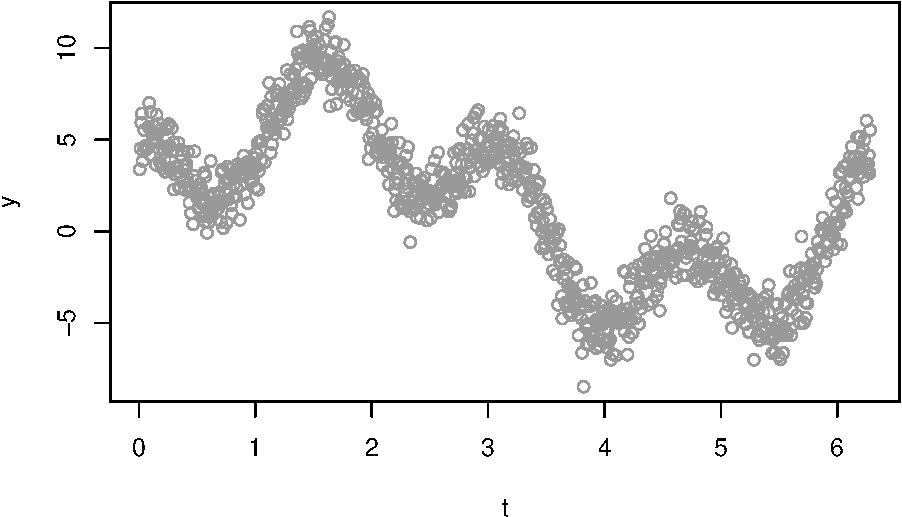
\includegraphics{김남윤_test_1_files/figure-latex/unnamed-chunk-3-1.pdf}
\#\#1-(4)번

\begin{Shaded}
\begin{Highlighting}[]
\NormalTok{X}\OtherTok{\textless{}{-}}\FunctionTok{cbind}\NormalTok{(}\DecValTok{1}\NormalTok{,x1,x2)}
\NormalTok{X}
\end{Highlighting}
\end{Shaded}

\begin{verbatim}
##                      x1          x2
##    [1,] 1  6.283144e-03  0.99968419
##    [2,] 1  1.256604e-02  0.99873696
##    [3,] 1  1.884844e-02  0.99715890
##    [4,] 1  2.513010e-02  0.99495102
##    [5,] 1  3.141076e-02  0.99211470
##    [6,] 1  3.769018e-02  0.98865174
##    [7,] 1  4.396812e-02  0.98456433
##    [8,] 1  5.024432e-02  0.97985505
##    [9,] 1  5.651853e-02  0.97452687
##   [10,] 1  6.279052e-02  0.96858316
##   [11,] 1  6.906003e-02  0.96202767
##   [12,] 1  7.532681e-02  0.95486454
##   [13,] 1  8.159061e-02  0.94709830
##   [14,] 1  8.785120e-02  0.93873386
##   [15,] 1  9.410831e-02  0.92977649
##   [16,] 1  1.003617e-01  0.92023185
##   [17,] 1  1.066112e-01  0.91010597
##   [18,] 1  1.128564e-01  0.89940525
##   [19,] 1  1.190972e-01  0.88813645
##   [20,] 1  1.253332e-01  0.87630668
##   [21,] 1  1.315644e-01  0.86392342
##   [22,] 1  1.377903e-01  0.85099448
##   [23,] 1  1.440108e-01  0.83752804
##   [24,] 1  1.502256e-01  0.82353260
##   [25,] 1  1.564345e-01  0.80901699
##   [26,] 1  1.626372e-01  0.79399040
##   [27,] 1  1.688334e-01  0.77846230
##   [28,] 1  1.750231e-01  0.76244251
##   [29,] 1  1.812058e-01  0.74594115
##   [30,] 1  1.873813e-01  0.72896863
##   [31,] 1  1.935495e-01  0.71153568
##   [32,] 1  1.997100e-01  0.69365331
##   [33,] 1  2.058626e-01  0.67533281
##   [34,] 1  2.120071e-01  0.65658576
##   [35,] 1  2.181432e-01  0.63742399
##   [36,] 1  2.242708e-01  0.61785961
##   [37,] 1  2.303894e-01  0.59790498
##   [38,] 1  2.364990e-01  0.57757270
##   [39,] 1  2.425992e-01  0.55687562
##   [40,] 1  2.486899e-01  0.53582679
##   [41,] 1  2.547707e-01  0.51443953
##   [42,] 1  2.608415e-01  0.49272734
##   [43,] 1  2.669020e-01  0.47070393
##   [44,] 1  2.729519e-01  0.44838322
##   [45,] 1  2.789911e-01  0.42577929
##   [46,] 1  2.850193e-01  0.40290644
##   [47,] 1  2.910362e-01  0.37977910
##   [48,] 1  2.970416e-01  0.35641188
##   [49,] 1  3.030353e-01  0.33281954
##   [50,] 1  3.090170e-01  0.30901699
##   [51,] 1  3.149865e-01  0.28501926
##   [52,] 1  3.209436e-01  0.26084151
##   [53,] 1  3.268880e-01  0.23649900
##   [54,] 1  3.328195e-01  0.21200711
##   [55,] 1  3.387379e-01  0.18738131
##   [56,] 1  3.446429e-01  0.16263717
##   [57,] 1  3.505343e-01  0.13779029
##   [58,] 1  3.564119e-01  0.11285638
##   [59,] 1  3.622754e-01  0.08785120
##   [60,] 1  3.681246e-01  0.06279052
##   [61,] 1  3.739592e-01  0.03769018
##   [62,] 1  3.797791e-01  0.01256604
##   [63,] 1  3.855840e-01 -0.01256604
##   [64,] 1  3.913737e-01 -0.03769018
##   [65,] 1  3.971479e-01 -0.06279052
##   [66,] 1  4.029064e-01 -0.08785120
##   [67,] 1  4.086491e-01 -0.11285638
##   [68,] 1  4.143756e-01 -0.13779029
##   [69,] 1  4.200857e-01 -0.16263717
##   [70,] 1  4.257793e-01 -0.18738131
##   [71,] 1  4.314560e-01 -0.21200711
##   [72,] 1  4.371158e-01 -0.23649900
##   [73,] 1  4.427582e-01 -0.26084151
##   [74,] 1  4.483832e-01 -0.28501926
##   [75,] 1  4.539905e-01 -0.30901699
##   [76,] 1  4.595799e-01 -0.33281954
##   [77,] 1  4.651511e-01 -0.35641188
##   [78,] 1  4.707039e-01 -0.37977910
##   [79,] 1  4.762382e-01 -0.40290644
##   [80,] 1  4.817537e-01 -0.42577929
##   [81,] 1  4.872501e-01 -0.44838322
##   [82,] 1  4.927273e-01 -0.47070393
##   [83,] 1  4.981851e-01 -0.49272734
##   [84,] 1  5.036232e-01 -0.51443953
##   [85,] 1  5.090414e-01 -0.53582679
##   [86,] 1  5.144395e-01 -0.55687562
##   [87,] 1  5.198173e-01 -0.57757270
##   [88,] 1  5.251746e-01 -0.59790498
##   [89,] 1  5.305112e-01 -0.61785961
##   [90,] 1  5.358268e-01 -0.63742399
##   [91,] 1  5.411213e-01 -0.65658576
##   [92,] 1  5.463943e-01 -0.67533281
##   [93,] 1  5.516459e-01 -0.69365331
##   [94,] 1  5.568756e-01 -0.71153568
##   [95,] 1  5.620834e-01 -0.72896863
##   [96,] 1  5.672689e-01 -0.74594115
##   [97,] 1  5.724321e-01 -0.76244251
##   [98,] 1  5.775727e-01 -0.77846230
##   [99,] 1  5.826905e-01 -0.79399040
##  [100,] 1  5.877853e-01 -0.80901699
##  [101,] 1  5.928568e-01 -0.82353260
##  [102,] 1  5.979050e-01 -0.83752804
##  [103,] 1  6.029295e-01 -0.85099448
##  [104,] 1  6.079303e-01 -0.86392342
##  [105,] 1  6.129071e-01 -0.87630668
##  [106,] 1  6.178596e-01 -0.88813645
##  [107,] 1  6.227878e-01 -0.89940525
##  [108,] 1  6.276914e-01 -0.91010597
##  [109,] 1  6.325702e-01 -0.92023185
##  [110,] 1  6.374240e-01 -0.92977649
##  [111,] 1  6.422527e-01 -0.93873386
##  [112,] 1  6.470560e-01 -0.94709830
##  [113,] 1  6.518337e-01 -0.95486454
##  [114,] 1  6.565858e-01 -0.96202767
##  [115,] 1  6.613119e-01 -0.96858316
##  [116,] 1  6.660119e-01 -0.97452687
##  [117,] 1  6.706856e-01 -0.97985505
##  [118,] 1  6.753328e-01 -0.98456433
##  [119,] 1  6.799534e-01 -0.98865174
##  [120,] 1  6.845471e-01 -0.99211470
##  [121,] 1  6.891138e-01 -0.99495102
##  [122,] 1  6.936533e-01 -0.99715890
##  [123,] 1  6.981654e-01 -0.99873696
##  [124,] 1  7.026500e-01 -0.99968419
##  [125,] 1  7.071068e-01 -1.00000000
##  [126,] 1  7.115357e-01 -0.99968419
##  [127,] 1  7.159365e-01 -0.99873696
##  [128,] 1  7.203090e-01 -0.99715890
##  [129,] 1  7.246531e-01 -0.99495102
##  [130,] 1  7.289686e-01 -0.99211470
##  [131,] 1  7.332553e-01 -0.98865174
##  [132,] 1  7.375131e-01 -0.98456433
##  [133,] 1  7.417418e-01 -0.97985505
##  [134,] 1  7.459411e-01 -0.97452687
##  [135,] 1  7.501111e-01 -0.96858316
##  [136,] 1  7.542514e-01 -0.96202767
##  [137,] 1  7.583619e-01 -0.95486454
##  [138,] 1  7.624425e-01 -0.94709830
##  [139,] 1  7.664930e-01 -0.93873386
##  [140,] 1  7.705132e-01 -0.92977649
##  [141,] 1  7.745031e-01 -0.92023185
##  [142,] 1  7.784623e-01 -0.91010597
##  [143,] 1  7.823908e-01 -0.89940525
##  [144,] 1  7.862884e-01 -0.88813645
##  [145,] 1  7.901550e-01 -0.87630668
##  [146,] 1  7.939904e-01 -0.86392342
##  [147,] 1  7.977944e-01 -0.85099448
##  [148,] 1  8.015670e-01 -0.83752804
##  [149,] 1  8.053079e-01 -0.82353260
##  [150,] 1  8.090170e-01 -0.80901699
##  [151,] 1  8.126942e-01 -0.79399040
##  [152,] 1  8.163393e-01 -0.77846230
##  [153,] 1  8.199521e-01 -0.76244251
##  [154,] 1  8.235326e-01 -0.74594115
##  [155,] 1  8.270806e-01 -0.72896863
##  [156,] 1  8.305959e-01 -0.71153568
##  [157,] 1  8.340784e-01 -0.69365331
##  [158,] 1  8.375280e-01 -0.67533281
##  [159,] 1  8.409446e-01 -0.65658576
##  [160,] 1  8.443279e-01 -0.63742399
##  [161,] 1  8.476779e-01 -0.61785961
##  [162,] 1  8.509945e-01 -0.59790498
##  [163,] 1  8.542774e-01 -0.57757270
##  [164,] 1  8.575267e-01 -0.55687562
##  [165,] 1  8.607420e-01 -0.53582679
##  [166,] 1  8.639234e-01 -0.51443953
##  [167,] 1  8.670707e-01 -0.49272734
##  [168,] 1  8.701838e-01 -0.47070393
##  [169,] 1  8.732625e-01 -0.44838322
##  [170,] 1  8.763067e-01 -0.42577929
##  [171,] 1  8.793163e-01 -0.40290644
##  [172,] 1  8.822912e-01 -0.37977910
##  [173,] 1  8.852313e-01 -0.35641188
##  [174,] 1  8.881364e-01 -0.33281954
##  [175,] 1  8.910065e-01 -0.30901699
##  [176,] 1  8.938414e-01 -0.28501926
##  [177,] 1  8.966410e-01 -0.26084151
##  [178,] 1  8.994053e-01 -0.23649900
##  [179,] 1  9.021340e-01 -0.21200711
##  [180,] 1  9.048271e-01 -0.18738131
##  [181,] 1  9.074844e-01 -0.16263717
##  [182,] 1  9.101060e-01 -0.13779029
##  [183,] 1  9.126916e-01 -0.11285638
##  [184,] 1  9.152412e-01 -0.08785120
##  [185,] 1  9.177546e-01 -0.06279052
##  [186,] 1  9.202318e-01 -0.03769018
##  [187,] 1  9.226727e-01 -0.01256604
##  [188,] 1  9.250772e-01  0.01256604
##  [189,] 1  9.274452e-01  0.03769018
##  [190,] 1  9.297765e-01  0.06279052
##  [191,] 1  9.320711e-01  0.08785120
##  [192,] 1  9.343289e-01  0.11285638
##  [193,] 1  9.365499e-01  0.13779029
##  [194,] 1  9.387339e-01  0.16263717
##  [195,] 1  9.408808e-01  0.18738131
##  [196,] 1  9.429905e-01  0.21200711
##  [197,] 1  9.450631e-01  0.23649900
##  [198,] 1  9.470983e-01  0.26084151
##  [199,] 1  9.490961e-01  0.28501926
##  [200,] 1  9.510565e-01  0.30901699
##  [201,] 1  9.529793e-01  0.33281954
##  [202,] 1  9.548645e-01  0.35641188
##  [203,] 1  9.567121e-01  0.37977910
##  [204,] 1  9.585218e-01  0.40290644
##  [205,] 1  9.602937e-01  0.42577929
##  [206,] 1  9.620277e-01  0.44838322
##  [207,] 1  9.637237e-01  0.47070393
##  [208,] 1  9.653816e-01  0.49272734
##  [209,] 1  9.670015e-01  0.51443953
##  [210,] 1  9.685832e-01  0.53582679
##  [211,] 1  9.701266e-01  0.55687562
##  [212,] 1  9.716317e-01  0.57757270
##  [213,] 1  9.730985e-01  0.59790498
##  [214,] 1  9.745269e-01  0.61785961
##  [215,] 1  9.759168e-01  0.63742399
##  [216,] 1  9.772681e-01  0.65658576
##  [217,] 1  9.785809e-01  0.67533281
##  [218,] 1  9.798551e-01  0.69365331
##  [219,] 1  9.810905e-01  0.71153568
##  [220,] 1  9.822873e-01  0.72896863
##  [221,] 1  9.834452e-01  0.74594115
##  [222,] 1  9.845643e-01  0.76244251
##  [223,] 1  9.856446e-01  0.77846230
##  [224,] 1  9.866859e-01  0.79399040
##  [225,] 1  9.876883e-01  0.80901699
##  [226,] 1  9.886517e-01  0.82353260
##  [227,] 1  9.895761e-01  0.83752804
##  [228,] 1  9.904614e-01  0.85099448
##  [229,] 1  9.913076e-01  0.86392342
##  [230,] 1  9.921147e-01  0.87630668
##  [231,] 1  9.928826e-01  0.88813645
##  [232,] 1  9.936113e-01  0.89940525
##  [233,] 1  9.943008e-01  0.91010597
##  [234,] 1  9.949510e-01  0.92023185
##  [235,] 1  9.955620e-01  0.92977649
##  [236,] 1  9.961336e-01  0.93873386
##  [237,] 1  9.966659e-01  0.94709830
##  [238,] 1  9.971589e-01  0.95486454
##  [239,] 1  9.976125e-01  0.96202767
##  [240,] 1  9.980267e-01  0.96858316
##  [241,] 1  9.984016e-01  0.97452687
##  [242,] 1  9.987370e-01  0.97985505
##  [243,] 1  9.990329e-01  0.98456433
##  [244,] 1  9.992895e-01  0.98865174
##  [245,] 1  9.995066e-01  0.99211470
##  [246,] 1  9.996842e-01  0.99495102
##  [247,] 1  9.998224e-01  0.99715890
##  [248,] 1  9.999210e-01  0.99873696
##  [249,] 1  9.999803e-01  0.99968419
##  [250,] 1  1.000000e+00  1.00000000
##  [251,] 1  9.999803e-01  0.99968419
##  [252,] 1  9.999210e-01  0.99873696
##  [253,] 1  9.998224e-01  0.99715890
##  [254,] 1  9.996842e-01  0.99495102
##  [255,] 1  9.995066e-01  0.99211470
##  [256,] 1  9.992895e-01  0.98865174
##  [257,] 1  9.990329e-01  0.98456433
##  [258,] 1  9.987370e-01  0.97985505
##  [259,] 1  9.984016e-01  0.97452687
##  [260,] 1  9.980267e-01  0.96858316
##  [261,] 1  9.976125e-01  0.96202767
##  [262,] 1  9.971589e-01  0.95486454
##  [263,] 1  9.966659e-01  0.94709830
##  [264,] 1  9.961336e-01  0.93873386
##  [265,] 1  9.955620e-01  0.92977649
##  [266,] 1  9.949510e-01  0.92023185
##  [267,] 1  9.943008e-01  0.91010597
##  [268,] 1  9.936113e-01  0.89940525
##  [269,] 1  9.928826e-01  0.88813645
##  [270,] 1  9.921147e-01  0.87630668
##  [271,] 1  9.913076e-01  0.86392342
##  [272,] 1  9.904614e-01  0.85099448
##  [273,] 1  9.895761e-01  0.83752804
##  [274,] 1  9.886517e-01  0.82353260
##  [275,] 1  9.876883e-01  0.80901699
##  [276,] 1  9.866859e-01  0.79399040
##  [277,] 1  9.856446e-01  0.77846230
##  [278,] 1  9.845643e-01  0.76244251
##  [279,] 1  9.834452e-01  0.74594115
##  [280,] 1  9.822873e-01  0.72896863
##  [281,] 1  9.810905e-01  0.71153568
##  [282,] 1  9.798551e-01  0.69365331
##  [283,] 1  9.785809e-01  0.67533281
##  [284,] 1  9.772681e-01  0.65658576
##  [285,] 1  9.759168e-01  0.63742399
##  [286,] 1  9.745269e-01  0.61785961
##  [287,] 1  9.730985e-01  0.59790498
##  [288,] 1  9.716317e-01  0.57757270
##  [289,] 1  9.701266e-01  0.55687562
##  [290,] 1  9.685832e-01  0.53582679
##  [291,] 1  9.670015e-01  0.51443953
##  [292,] 1  9.653816e-01  0.49272734
##  [293,] 1  9.637237e-01  0.47070393
##  [294,] 1  9.620277e-01  0.44838322
##  [295,] 1  9.602937e-01  0.42577929
##  [296,] 1  9.585218e-01  0.40290644
##  [297,] 1  9.567121e-01  0.37977910
##  [298,] 1  9.548645e-01  0.35641188
##  [299,] 1  9.529793e-01  0.33281954
##  [300,] 1  9.510565e-01  0.30901699
##  [301,] 1  9.490961e-01  0.28501926
##  [302,] 1  9.470983e-01  0.26084151
##  [303,] 1  9.450631e-01  0.23649900
##  [304,] 1  9.429905e-01  0.21200711
##  [305,] 1  9.408808e-01  0.18738131
##  [306,] 1  9.387339e-01  0.16263717
##  [307,] 1  9.365499e-01  0.13779029
##  [308,] 1  9.343289e-01  0.11285638
##  [309,] 1  9.320711e-01  0.08785120
##  [310,] 1  9.297765e-01  0.06279052
##  [311,] 1  9.274452e-01  0.03769018
##  [312,] 1  9.250772e-01  0.01256604
##  [313,] 1  9.226727e-01 -0.01256604
##  [314,] 1  9.202318e-01 -0.03769018
##  [315,] 1  9.177546e-01 -0.06279052
##  [316,] 1  9.152412e-01 -0.08785120
##  [317,] 1  9.126916e-01 -0.11285638
##  [318,] 1  9.101060e-01 -0.13779029
##  [319,] 1  9.074844e-01 -0.16263717
##  [320,] 1  9.048271e-01 -0.18738131
##  [321,] 1  9.021340e-01 -0.21200711
##  [322,] 1  8.994053e-01 -0.23649900
##  [323,] 1  8.966410e-01 -0.26084151
##  [324,] 1  8.938414e-01 -0.28501926
##  [325,] 1  8.910065e-01 -0.30901699
##  [326,] 1  8.881364e-01 -0.33281954
##  [327,] 1  8.852313e-01 -0.35641188
##  [328,] 1  8.822912e-01 -0.37977910
##  [329,] 1  8.793163e-01 -0.40290644
##  [330,] 1  8.763067e-01 -0.42577929
##  [331,] 1  8.732625e-01 -0.44838322
##  [332,] 1  8.701838e-01 -0.47070393
##  [333,] 1  8.670707e-01 -0.49272734
##  [334,] 1  8.639234e-01 -0.51443953
##  [335,] 1  8.607420e-01 -0.53582679
##  [336,] 1  8.575267e-01 -0.55687562
##  [337,] 1  8.542774e-01 -0.57757270
##  [338,] 1  8.509945e-01 -0.59790498
##  [339,] 1  8.476779e-01 -0.61785961
##  [340,] 1  8.443279e-01 -0.63742399
##  [341,] 1  8.409446e-01 -0.65658576
##  [342,] 1  8.375280e-01 -0.67533281
##  [343,] 1  8.340784e-01 -0.69365331
##  [344,] 1  8.305959e-01 -0.71153568
##  [345,] 1  8.270806e-01 -0.72896863
##  [346,] 1  8.235326e-01 -0.74594115
##  [347,] 1  8.199521e-01 -0.76244251
##  [348,] 1  8.163393e-01 -0.77846230
##  [349,] 1  8.126942e-01 -0.79399040
##  [350,] 1  8.090170e-01 -0.80901699
##  [351,] 1  8.053079e-01 -0.82353260
##  [352,] 1  8.015670e-01 -0.83752804
##  [353,] 1  7.977944e-01 -0.85099448
##  [354,] 1  7.939904e-01 -0.86392342
##  [355,] 1  7.901550e-01 -0.87630668
##  [356,] 1  7.862884e-01 -0.88813645
##  [357,] 1  7.823908e-01 -0.89940525
##  [358,] 1  7.784623e-01 -0.91010597
##  [359,] 1  7.745031e-01 -0.92023185
##  [360,] 1  7.705132e-01 -0.92977649
##  [361,] 1  7.664930e-01 -0.93873386
##  [362,] 1  7.624425e-01 -0.94709830
##  [363,] 1  7.583619e-01 -0.95486454
##  [364,] 1  7.542514e-01 -0.96202767
##  [365,] 1  7.501111e-01 -0.96858316
##  [366,] 1  7.459411e-01 -0.97452687
##  [367,] 1  7.417418e-01 -0.97985505
##  [368,] 1  7.375131e-01 -0.98456433
##  [369,] 1  7.332553e-01 -0.98865174
##  [370,] 1  7.289686e-01 -0.99211470
##  [371,] 1  7.246531e-01 -0.99495102
##  [372,] 1  7.203090e-01 -0.99715890
##  [373,] 1  7.159365e-01 -0.99873696
##  [374,] 1  7.115357e-01 -0.99968419
##  [375,] 1  7.071068e-01 -1.00000000
##  [376,] 1  7.026500e-01 -0.99968419
##  [377,] 1  6.981654e-01 -0.99873696
##  [378,] 1  6.936533e-01 -0.99715890
##  [379,] 1  6.891138e-01 -0.99495102
##  [380,] 1  6.845471e-01 -0.99211470
##  [381,] 1  6.799534e-01 -0.98865174
##  [382,] 1  6.753328e-01 -0.98456433
##  [383,] 1  6.706856e-01 -0.97985505
##  [384,] 1  6.660119e-01 -0.97452687
##  [385,] 1  6.613119e-01 -0.96858316
##  [386,] 1  6.565858e-01 -0.96202767
##  [387,] 1  6.518337e-01 -0.95486454
##  [388,] 1  6.470560e-01 -0.94709830
##  [389,] 1  6.422527e-01 -0.93873386
##  [390,] 1  6.374240e-01 -0.92977649
##  [391,] 1  6.325702e-01 -0.92023185
##  [392,] 1  6.276914e-01 -0.91010597
##  [393,] 1  6.227878e-01 -0.89940525
##  [394,] 1  6.178596e-01 -0.88813645
##  [395,] 1  6.129071e-01 -0.87630668
##  [396,] 1  6.079303e-01 -0.86392342
##  [397,] 1  6.029295e-01 -0.85099448
##  [398,] 1  5.979050e-01 -0.83752804
##  [399,] 1  5.928568e-01 -0.82353260
##  [400,] 1  5.877853e-01 -0.80901699
##  [401,] 1  5.826905e-01 -0.79399040
##  [402,] 1  5.775727e-01 -0.77846230
##  [403,] 1  5.724321e-01 -0.76244251
##  [404,] 1  5.672689e-01 -0.74594115
##  [405,] 1  5.620834e-01 -0.72896863
##  [406,] 1  5.568756e-01 -0.71153568
##  [407,] 1  5.516459e-01 -0.69365331
##  [408,] 1  5.463943e-01 -0.67533281
##  [409,] 1  5.411213e-01 -0.65658576
##  [410,] 1  5.358268e-01 -0.63742399
##  [411,] 1  5.305112e-01 -0.61785961
##  [412,] 1  5.251746e-01 -0.59790498
##  [413,] 1  5.198173e-01 -0.57757270
##  [414,] 1  5.144395e-01 -0.55687562
##  [415,] 1  5.090414e-01 -0.53582679
##  [416,] 1  5.036232e-01 -0.51443953
##  [417,] 1  4.981851e-01 -0.49272734
##  [418,] 1  4.927273e-01 -0.47070393
##  [419,] 1  4.872501e-01 -0.44838322
##  [420,] 1  4.817537e-01 -0.42577929
##  [421,] 1  4.762382e-01 -0.40290644
##  [422,] 1  4.707039e-01 -0.37977910
##  [423,] 1  4.651511e-01 -0.35641188
##  [424,] 1  4.595799e-01 -0.33281954
##  [425,] 1  4.539905e-01 -0.30901699
##  [426,] 1  4.483832e-01 -0.28501926
##  [427,] 1  4.427582e-01 -0.26084151
##  [428,] 1  4.371158e-01 -0.23649900
##  [429,] 1  4.314560e-01 -0.21200711
##  [430,] 1  4.257793e-01 -0.18738131
##  [431,] 1  4.200857e-01 -0.16263717
##  [432,] 1  4.143756e-01 -0.13779029
##  [433,] 1  4.086491e-01 -0.11285638
##  [434,] 1  4.029064e-01 -0.08785120
##  [435,] 1  3.971479e-01 -0.06279052
##  [436,] 1  3.913737e-01 -0.03769018
##  [437,] 1  3.855840e-01 -0.01256604
##  [438,] 1  3.797791e-01  0.01256604
##  [439,] 1  3.739592e-01  0.03769018
##  [440,] 1  3.681246e-01  0.06279052
##  [441,] 1  3.622754e-01  0.08785120
##  [442,] 1  3.564119e-01  0.11285638
##  [443,] 1  3.505343e-01  0.13779029
##  [444,] 1  3.446429e-01  0.16263717
##  [445,] 1  3.387379e-01  0.18738131
##  [446,] 1  3.328195e-01  0.21200711
##  [447,] 1  3.268880e-01  0.23649900
##  [448,] 1  3.209436e-01  0.26084151
##  [449,] 1  3.149865e-01  0.28501926
##  [450,] 1  3.090170e-01  0.30901699
##  [451,] 1  3.030353e-01  0.33281954
##  [452,] 1  2.970416e-01  0.35641188
##  [453,] 1  2.910362e-01  0.37977910
##  [454,] 1  2.850193e-01  0.40290644
##  [455,] 1  2.789911e-01  0.42577929
##  [456,] 1  2.729519e-01  0.44838322
##  [457,] 1  2.669020e-01  0.47070393
##  [458,] 1  2.608415e-01  0.49272734
##  [459,] 1  2.547707e-01  0.51443953
##  [460,] 1  2.486899e-01  0.53582679
##  [461,] 1  2.425992e-01  0.55687562
##  [462,] 1  2.364990e-01  0.57757270
##  [463,] 1  2.303894e-01  0.59790498
##  [464,] 1  2.242708e-01  0.61785961
##  [465,] 1  2.181432e-01  0.63742399
##  [466,] 1  2.120071e-01  0.65658576
##  [467,] 1  2.058626e-01  0.67533281
##  [468,] 1  1.997100e-01  0.69365331
##  [469,] 1  1.935495e-01  0.71153568
##  [470,] 1  1.873813e-01  0.72896863
##  [471,] 1  1.812058e-01  0.74594115
##  [472,] 1  1.750231e-01  0.76244251
##  [473,] 1  1.688334e-01  0.77846230
##  [474,] 1  1.626372e-01  0.79399040
##  [475,] 1  1.564345e-01  0.80901699
##  [476,] 1  1.502256e-01  0.82353260
##  [477,] 1  1.440108e-01  0.83752804
##  [478,] 1  1.377903e-01  0.85099448
##  [479,] 1  1.315644e-01  0.86392342
##  [480,] 1  1.253332e-01  0.87630668
##  [481,] 1  1.190972e-01  0.88813645
##  [482,] 1  1.128564e-01  0.89940525
##  [483,] 1  1.066112e-01  0.91010597
##  [484,] 1  1.003617e-01  0.92023185
##  [485,] 1  9.410831e-02  0.92977649
##  [486,] 1  8.785120e-02  0.93873386
##  [487,] 1  8.159061e-02  0.94709830
##  [488,] 1  7.532681e-02  0.95486454
##  [489,] 1  6.906003e-02  0.96202767
##  [490,] 1  6.279052e-02  0.96858316
##  [491,] 1  5.651853e-02  0.97452687
##  [492,] 1  5.024432e-02  0.97985505
##  [493,] 1  4.396812e-02  0.98456433
##  [494,] 1  3.769018e-02  0.98865174
##  [495,] 1  3.141076e-02  0.99211470
##  [496,] 1  2.513010e-02  0.99495102
##  [497,] 1  1.884844e-02  0.99715890
##  [498,] 1  1.256604e-02  0.99873696
##  [499,] 1  6.283144e-03  0.99968419
##  [500,] 1  1.224647e-16  1.00000000
##  [501,] 1 -6.283144e-03  0.99968419
##  [502,] 1 -1.256604e-02  0.99873696
##  [503,] 1 -1.884844e-02  0.99715890
##  [504,] 1 -2.513010e-02  0.99495102
##  [505,] 1 -3.141076e-02  0.99211470
##  [506,] 1 -3.769018e-02  0.98865174
##  [507,] 1 -4.396812e-02  0.98456433
##  [508,] 1 -5.024432e-02  0.97985505
##  [509,] 1 -5.651853e-02  0.97452687
##  [510,] 1 -6.279052e-02  0.96858316
##  [511,] 1 -6.906003e-02  0.96202767
##  [512,] 1 -7.532681e-02  0.95486454
##  [513,] 1 -8.159061e-02  0.94709830
##  [514,] 1 -8.785120e-02  0.93873386
##  [515,] 1 -9.410831e-02  0.92977649
##  [516,] 1 -1.003617e-01  0.92023185
##  [517,] 1 -1.066112e-01  0.91010597
##  [518,] 1 -1.128564e-01  0.89940525
##  [519,] 1 -1.190972e-01  0.88813645
##  [520,] 1 -1.253332e-01  0.87630668
##  [521,] 1 -1.315644e-01  0.86392342
##  [522,] 1 -1.377903e-01  0.85099448
##  [523,] 1 -1.440108e-01  0.83752804
##  [524,] 1 -1.502256e-01  0.82353260
##  [525,] 1 -1.564345e-01  0.80901699
##  [526,] 1 -1.626372e-01  0.79399040
##  [527,] 1 -1.688334e-01  0.77846230
##  [528,] 1 -1.750231e-01  0.76244251
##  [529,] 1 -1.812058e-01  0.74594115
##  [530,] 1 -1.873813e-01  0.72896863
##  [531,] 1 -1.935495e-01  0.71153568
##  [532,] 1 -1.997100e-01  0.69365331
##  [533,] 1 -2.058626e-01  0.67533281
##  [534,] 1 -2.120071e-01  0.65658576
##  [535,] 1 -2.181432e-01  0.63742399
##  [536,] 1 -2.242708e-01  0.61785961
##  [537,] 1 -2.303894e-01  0.59790498
##  [538,] 1 -2.364990e-01  0.57757270
##  [539,] 1 -2.425992e-01  0.55687562
##  [540,] 1 -2.486899e-01  0.53582679
##  [541,] 1 -2.547707e-01  0.51443953
##  [542,] 1 -2.608415e-01  0.49272734
##  [543,] 1 -2.669020e-01  0.47070393
##  [544,] 1 -2.729519e-01  0.44838322
##  [545,] 1 -2.789911e-01  0.42577929
##  [546,] 1 -2.850193e-01  0.40290644
##  [547,] 1 -2.910362e-01  0.37977910
##  [548,] 1 -2.970416e-01  0.35641188
##  [549,] 1 -3.030353e-01  0.33281954
##  [550,] 1 -3.090170e-01  0.30901699
##  [551,] 1 -3.149865e-01  0.28501926
##  [552,] 1 -3.209436e-01  0.26084151
##  [553,] 1 -3.268880e-01  0.23649900
##  [554,] 1 -3.328195e-01  0.21200711
##  [555,] 1 -3.387379e-01  0.18738131
##  [556,] 1 -3.446429e-01  0.16263717
##  [557,] 1 -3.505343e-01  0.13779029
##  [558,] 1 -3.564119e-01  0.11285638
##  [559,] 1 -3.622754e-01  0.08785120
##  [560,] 1 -3.681246e-01  0.06279052
##  [561,] 1 -3.739592e-01  0.03769018
##  [562,] 1 -3.797791e-01  0.01256604
##  [563,] 1 -3.855840e-01 -0.01256604
##  [564,] 1 -3.913737e-01 -0.03769018
##  [565,] 1 -3.971479e-01 -0.06279052
##  [566,] 1 -4.029064e-01 -0.08785120
##  [567,] 1 -4.086491e-01 -0.11285638
##  [568,] 1 -4.143756e-01 -0.13779029
##  [569,] 1 -4.200857e-01 -0.16263717
##  [570,] 1 -4.257793e-01 -0.18738131
##  [571,] 1 -4.314560e-01 -0.21200711
##  [572,] 1 -4.371158e-01 -0.23649900
##  [573,] 1 -4.427582e-01 -0.26084151
##  [574,] 1 -4.483832e-01 -0.28501926
##  [575,] 1 -4.539905e-01 -0.30901699
##  [576,] 1 -4.595799e-01 -0.33281954
##  [577,] 1 -4.651511e-01 -0.35641188
##  [578,] 1 -4.707039e-01 -0.37977910
##  [579,] 1 -4.762382e-01 -0.40290644
##  [580,] 1 -4.817537e-01 -0.42577929
##  [581,] 1 -4.872501e-01 -0.44838322
##  [582,] 1 -4.927273e-01 -0.47070393
##  [583,] 1 -4.981851e-01 -0.49272734
##  [584,] 1 -5.036232e-01 -0.51443953
##  [585,] 1 -5.090414e-01 -0.53582679
##  [586,] 1 -5.144395e-01 -0.55687562
##  [587,] 1 -5.198173e-01 -0.57757270
##  [588,] 1 -5.251746e-01 -0.59790498
##  [589,] 1 -5.305112e-01 -0.61785961
##  [590,] 1 -5.358268e-01 -0.63742399
##  [591,] 1 -5.411213e-01 -0.65658576
##  [592,] 1 -5.463943e-01 -0.67533281
##  [593,] 1 -5.516459e-01 -0.69365331
##  [594,] 1 -5.568756e-01 -0.71153568
##  [595,] 1 -5.620834e-01 -0.72896863
##  [596,] 1 -5.672689e-01 -0.74594115
##  [597,] 1 -5.724321e-01 -0.76244251
##  [598,] 1 -5.775727e-01 -0.77846230
##  [599,] 1 -5.826905e-01 -0.79399040
##  [600,] 1 -5.877853e-01 -0.80901699
##  [601,] 1 -5.928568e-01 -0.82353260
##  [602,] 1 -5.979050e-01 -0.83752804
##  [603,] 1 -6.029295e-01 -0.85099448
##  [604,] 1 -6.079303e-01 -0.86392342
##  [605,] 1 -6.129071e-01 -0.87630668
##  [606,] 1 -6.178596e-01 -0.88813645
##  [607,] 1 -6.227878e-01 -0.89940525
##  [608,] 1 -6.276914e-01 -0.91010597
##  [609,] 1 -6.325702e-01 -0.92023185
##  [610,] 1 -6.374240e-01 -0.92977649
##  [611,] 1 -6.422527e-01 -0.93873386
##  [612,] 1 -6.470560e-01 -0.94709830
##  [613,] 1 -6.518337e-01 -0.95486454
##  [614,] 1 -6.565858e-01 -0.96202767
##  [615,] 1 -6.613119e-01 -0.96858316
##  [616,] 1 -6.660119e-01 -0.97452687
##  [617,] 1 -6.706856e-01 -0.97985505
##  [618,] 1 -6.753328e-01 -0.98456433
##  [619,] 1 -6.799534e-01 -0.98865174
##  [620,] 1 -6.845471e-01 -0.99211470
##  [621,] 1 -6.891138e-01 -0.99495102
##  [622,] 1 -6.936533e-01 -0.99715890
##  [623,] 1 -6.981654e-01 -0.99873696
##  [624,] 1 -7.026500e-01 -0.99968419
##  [625,] 1 -7.071068e-01 -1.00000000
##  [626,] 1 -7.115357e-01 -0.99968419
##  [627,] 1 -7.159365e-01 -0.99873696
##  [628,] 1 -7.203090e-01 -0.99715890
##  [629,] 1 -7.246531e-01 -0.99495102
##  [630,] 1 -7.289686e-01 -0.99211470
##  [631,] 1 -7.332553e-01 -0.98865174
##  [632,] 1 -7.375131e-01 -0.98456433
##  [633,] 1 -7.417418e-01 -0.97985505
##  [634,] 1 -7.459411e-01 -0.97452687
##  [635,] 1 -7.501111e-01 -0.96858316
##  [636,] 1 -7.542514e-01 -0.96202767
##  [637,] 1 -7.583619e-01 -0.95486454
##  [638,] 1 -7.624425e-01 -0.94709830
##  [639,] 1 -7.664930e-01 -0.93873386
##  [640,] 1 -7.705132e-01 -0.92977649
##  [641,] 1 -7.745031e-01 -0.92023185
##  [642,] 1 -7.784623e-01 -0.91010597
##  [643,] 1 -7.823908e-01 -0.89940525
##  [644,] 1 -7.862884e-01 -0.88813645
##  [645,] 1 -7.901550e-01 -0.87630668
##  [646,] 1 -7.939904e-01 -0.86392342
##  [647,] 1 -7.977944e-01 -0.85099448
##  [648,] 1 -8.015670e-01 -0.83752804
##  [649,] 1 -8.053079e-01 -0.82353260
##  [650,] 1 -8.090170e-01 -0.80901699
##  [651,] 1 -8.126942e-01 -0.79399040
##  [652,] 1 -8.163393e-01 -0.77846230
##  [653,] 1 -8.199521e-01 -0.76244251
##  [654,] 1 -8.235326e-01 -0.74594115
##  [655,] 1 -8.270806e-01 -0.72896863
##  [656,] 1 -8.305959e-01 -0.71153568
##  [657,] 1 -8.340784e-01 -0.69365331
##  [658,] 1 -8.375280e-01 -0.67533281
##  [659,] 1 -8.409446e-01 -0.65658576
##  [660,] 1 -8.443279e-01 -0.63742399
##  [661,] 1 -8.476779e-01 -0.61785961
##  [662,] 1 -8.509945e-01 -0.59790498
##  [663,] 1 -8.542774e-01 -0.57757270
##  [664,] 1 -8.575267e-01 -0.55687562
##  [665,] 1 -8.607420e-01 -0.53582679
##  [666,] 1 -8.639234e-01 -0.51443953
##  [667,] 1 -8.670707e-01 -0.49272734
##  [668,] 1 -8.701838e-01 -0.47070393
##  [669,] 1 -8.732625e-01 -0.44838322
##  [670,] 1 -8.763067e-01 -0.42577929
##  [671,] 1 -8.793163e-01 -0.40290644
##  [672,] 1 -8.822912e-01 -0.37977910
##  [673,] 1 -8.852313e-01 -0.35641188
##  [674,] 1 -8.881364e-01 -0.33281954
##  [675,] 1 -8.910065e-01 -0.30901699
##  [676,] 1 -8.938414e-01 -0.28501926
##  [677,] 1 -8.966410e-01 -0.26084151
##  [678,] 1 -8.994053e-01 -0.23649900
##  [679,] 1 -9.021340e-01 -0.21200711
##  [680,] 1 -9.048271e-01 -0.18738131
##  [681,] 1 -9.074844e-01 -0.16263717
##  [682,] 1 -9.101060e-01 -0.13779029
##  [683,] 1 -9.126916e-01 -0.11285638
##  [684,] 1 -9.152412e-01 -0.08785120
##  [685,] 1 -9.177546e-01 -0.06279052
##  [686,] 1 -9.202318e-01 -0.03769018
##  [687,] 1 -9.226727e-01 -0.01256604
##  [688,] 1 -9.250772e-01  0.01256604
##  [689,] 1 -9.274452e-01  0.03769018
##  [690,] 1 -9.297765e-01  0.06279052
##  [691,] 1 -9.320711e-01  0.08785120
##  [692,] 1 -9.343289e-01  0.11285638
##  [693,] 1 -9.365499e-01  0.13779029
##  [694,] 1 -9.387339e-01  0.16263717
##  [695,] 1 -9.408808e-01  0.18738131
##  [696,] 1 -9.429905e-01  0.21200711
##  [697,] 1 -9.450631e-01  0.23649900
##  [698,] 1 -9.470983e-01  0.26084151
##  [699,] 1 -9.490961e-01  0.28501926
##  [700,] 1 -9.510565e-01  0.30901699
##  [701,] 1 -9.529793e-01  0.33281954
##  [702,] 1 -9.548645e-01  0.35641188
##  [703,] 1 -9.567121e-01  0.37977910
##  [704,] 1 -9.585218e-01  0.40290644
##  [705,] 1 -9.602937e-01  0.42577929
##  [706,] 1 -9.620277e-01  0.44838322
##  [707,] 1 -9.637237e-01  0.47070393
##  [708,] 1 -9.653816e-01  0.49272734
##  [709,] 1 -9.670015e-01  0.51443953
##  [710,] 1 -9.685832e-01  0.53582679
##  [711,] 1 -9.701266e-01  0.55687562
##  [712,] 1 -9.716317e-01  0.57757270
##  [713,] 1 -9.730985e-01  0.59790498
##  [714,] 1 -9.745269e-01  0.61785961
##  [715,] 1 -9.759168e-01  0.63742399
##  [716,] 1 -9.772681e-01  0.65658576
##  [717,] 1 -9.785809e-01  0.67533281
##  [718,] 1 -9.798551e-01  0.69365331
##  [719,] 1 -9.810905e-01  0.71153568
##  [720,] 1 -9.822873e-01  0.72896863
##  [721,] 1 -9.834452e-01  0.74594115
##  [722,] 1 -9.845643e-01  0.76244251
##  [723,] 1 -9.856446e-01  0.77846230
##  [724,] 1 -9.866859e-01  0.79399040
##  [725,] 1 -9.876883e-01  0.80901699
##  [726,] 1 -9.886517e-01  0.82353260
##  [727,] 1 -9.895761e-01  0.83752804
##  [728,] 1 -9.904614e-01  0.85099448
##  [729,] 1 -9.913076e-01  0.86392342
##  [730,] 1 -9.921147e-01  0.87630668
##  [731,] 1 -9.928826e-01  0.88813645
##  [732,] 1 -9.936113e-01  0.89940525
##  [733,] 1 -9.943008e-01  0.91010597
##  [734,] 1 -9.949510e-01  0.92023185
##  [735,] 1 -9.955620e-01  0.92977649
##  [736,] 1 -9.961336e-01  0.93873386
##  [737,] 1 -9.966659e-01  0.94709830
##  [738,] 1 -9.971589e-01  0.95486454
##  [739,] 1 -9.976125e-01  0.96202767
##  [740,] 1 -9.980267e-01  0.96858316
##  [741,] 1 -9.984016e-01  0.97452687
##  [742,] 1 -9.987370e-01  0.97985505
##  [743,] 1 -9.990329e-01  0.98456433
##  [744,] 1 -9.992895e-01  0.98865174
##  [745,] 1 -9.995066e-01  0.99211470
##  [746,] 1 -9.996842e-01  0.99495102
##  [747,] 1 -9.998224e-01  0.99715890
##  [748,] 1 -9.999210e-01  0.99873696
##  [749,] 1 -9.999803e-01  0.99968419
##  [750,] 1 -1.000000e+00  1.00000000
##  [751,] 1 -9.999803e-01  0.99968419
##  [752,] 1 -9.999210e-01  0.99873696
##  [753,] 1 -9.998224e-01  0.99715890
##  [754,] 1 -9.996842e-01  0.99495102
##  [755,] 1 -9.995066e-01  0.99211470
##  [756,] 1 -9.992895e-01  0.98865174
##  [757,] 1 -9.990329e-01  0.98456433
##  [758,] 1 -9.987370e-01  0.97985505
##  [759,] 1 -9.984016e-01  0.97452687
##  [760,] 1 -9.980267e-01  0.96858316
##  [761,] 1 -9.976125e-01  0.96202767
##  [762,] 1 -9.971589e-01  0.95486454
##  [763,] 1 -9.966659e-01  0.94709830
##  [764,] 1 -9.961336e-01  0.93873386
##  [765,] 1 -9.955620e-01  0.92977649
##  [766,] 1 -9.949510e-01  0.92023185
##  [767,] 1 -9.943008e-01  0.91010597
##  [768,] 1 -9.936113e-01  0.89940525
##  [769,] 1 -9.928826e-01  0.88813645
##  [770,] 1 -9.921147e-01  0.87630668
##  [771,] 1 -9.913076e-01  0.86392342
##  [772,] 1 -9.904614e-01  0.85099448
##  [773,] 1 -9.895761e-01  0.83752804
##  [774,] 1 -9.886517e-01  0.82353260
##  [775,] 1 -9.876883e-01  0.80901699
##  [776,] 1 -9.866859e-01  0.79399040
##  [777,] 1 -9.856446e-01  0.77846230
##  [778,] 1 -9.845643e-01  0.76244251
##  [779,] 1 -9.834452e-01  0.74594115
##  [780,] 1 -9.822873e-01  0.72896863
##  [781,] 1 -9.810905e-01  0.71153568
##  [782,] 1 -9.798551e-01  0.69365331
##  [783,] 1 -9.785809e-01  0.67533281
##  [784,] 1 -9.772681e-01  0.65658576
##  [785,] 1 -9.759168e-01  0.63742399
##  [786,] 1 -9.745269e-01  0.61785961
##  [787,] 1 -9.730985e-01  0.59790498
##  [788,] 1 -9.716317e-01  0.57757270
##  [789,] 1 -9.701266e-01  0.55687562
##  [790,] 1 -9.685832e-01  0.53582679
##  [791,] 1 -9.670015e-01  0.51443953
##  [792,] 1 -9.653816e-01  0.49272734
##  [793,] 1 -9.637237e-01  0.47070393
##  [794,] 1 -9.620277e-01  0.44838322
##  [795,] 1 -9.602937e-01  0.42577929
##  [796,] 1 -9.585218e-01  0.40290644
##  [797,] 1 -9.567121e-01  0.37977910
##  [798,] 1 -9.548645e-01  0.35641188
##  [799,] 1 -9.529793e-01  0.33281954
##  [800,] 1 -9.510565e-01  0.30901699
##  [801,] 1 -9.490961e-01  0.28501926
##  [802,] 1 -9.470983e-01  0.26084151
##  [803,] 1 -9.450631e-01  0.23649900
##  [804,] 1 -9.429905e-01  0.21200711
##  [805,] 1 -9.408808e-01  0.18738131
##  [806,] 1 -9.387339e-01  0.16263717
##  [807,] 1 -9.365499e-01  0.13779029
##  [808,] 1 -9.343289e-01  0.11285638
##  [809,] 1 -9.320711e-01  0.08785120
##  [810,] 1 -9.297765e-01  0.06279052
##  [811,] 1 -9.274452e-01  0.03769018
##  [812,] 1 -9.250772e-01  0.01256604
##  [813,] 1 -9.226727e-01 -0.01256604
##  [814,] 1 -9.202318e-01 -0.03769018
##  [815,] 1 -9.177546e-01 -0.06279052
##  [816,] 1 -9.152412e-01 -0.08785120
##  [817,] 1 -9.126916e-01 -0.11285638
##  [818,] 1 -9.101060e-01 -0.13779029
##  [819,] 1 -9.074844e-01 -0.16263717
##  [820,] 1 -9.048271e-01 -0.18738131
##  [821,] 1 -9.021340e-01 -0.21200711
##  [822,] 1 -8.994053e-01 -0.23649900
##  [823,] 1 -8.966410e-01 -0.26084151
##  [824,] 1 -8.938414e-01 -0.28501926
##  [825,] 1 -8.910065e-01 -0.30901699
##  [826,] 1 -8.881364e-01 -0.33281954
##  [827,] 1 -8.852313e-01 -0.35641188
##  [828,] 1 -8.822912e-01 -0.37977910
##  [829,] 1 -8.793163e-01 -0.40290644
##  [830,] 1 -8.763067e-01 -0.42577929
##  [831,] 1 -8.732625e-01 -0.44838322
##  [832,] 1 -8.701838e-01 -0.47070393
##  [833,] 1 -8.670707e-01 -0.49272734
##  [834,] 1 -8.639234e-01 -0.51443953
##  [835,] 1 -8.607420e-01 -0.53582679
##  [836,] 1 -8.575267e-01 -0.55687562
##  [837,] 1 -8.542774e-01 -0.57757270
##  [838,] 1 -8.509945e-01 -0.59790498
##  [839,] 1 -8.476779e-01 -0.61785961
##  [840,] 1 -8.443279e-01 -0.63742399
##  [841,] 1 -8.409446e-01 -0.65658576
##  [842,] 1 -8.375280e-01 -0.67533281
##  [843,] 1 -8.340784e-01 -0.69365331
##  [844,] 1 -8.305959e-01 -0.71153568
##  [845,] 1 -8.270806e-01 -0.72896863
##  [846,] 1 -8.235326e-01 -0.74594115
##  [847,] 1 -8.199521e-01 -0.76244251
##  [848,] 1 -8.163393e-01 -0.77846230
##  [849,] 1 -8.126942e-01 -0.79399040
##  [850,] 1 -8.090170e-01 -0.80901699
##  [851,] 1 -8.053079e-01 -0.82353260
##  [852,] 1 -8.015670e-01 -0.83752804
##  [853,] 1 -7.977944e-01 -0.85099448
##  [854,] 1 -7.939904e-01 -0.86392342
##  [855,] 1 -7.901550e-01 -0.87630668
##  [856,] 1 -7.862884e-01 -0.88813645
##  [857,] 1 -7.823908e-01 -0.89940525
##  [858,] 1 -7.784623e-01 -0.91010597
##  [859,] 1 -7.745031e-01 -0.92023185
##  [860,] 1 -7.705132e-01 -0.92977649
##  [861,] 1 -7.664930e-01 -0.93873386
##  [862,] 1 -7.624425e-01 -0.94709830
##  [863,] 1 -7.583619e-01 -0.95486454
##  [864,] 1 -7.542514e-01 -0.96202767
##  [865,] 1 -7.501111e-01 -0.96858316
##  [866,] 1 -7.459411e-01 -0.97452687
##  [867,] 1 -7.417418e-01 -0.97985505
##  [868,] 1 -7.375131e-01 -0.98456433
##  [869,] 1 -7.332553e-01 -0.98865174
##  [870,] 1 -7.289686e-01 -0.99211470
##  [871,] 1 -7.246531e-01 -0.99495102
##  [872,] 1 -7.203090e-01 -0.99715890
##  [873,] 1 -7.159365e-01 -0.99873696
##  [874,] 1 -7.115357e-01 -0.99968419
##  [875,] 1 -7.071068e-01 -1.00000000
##  [876,] 1 -7.026500e-01 -0.99968419
##  [877,] 1 -6.981654e-01 -0.99873696
##  [878,] 1 -6.936533e-01 -0.99715890
##  [879,] 1 -6.891138e-01 -0.99495102
##  [880,] 1 -6.845471e-01 -0.99211470
##  [881,] 1 -6.799534e-01 -0.98865174
##  [882,] 1 -6.753328e-01 -0.98456433
##  [883,] 1 -6.706856e-01 -0.97985505
##  [884,] 1 -6.660119e-01 -0.97452687
##  [885,] 1 -6.613119e-01 -0.96858316
##  [886,] 1 -6.565858e-01 -0.96202767
##  [887,] 1 -6.518337e-01 -0.95486454
##  [888,] 1 -6.470560e-01 -0.94709830
##  [889,] 1 -6.422527e-01 -0.93873386
##  [890,] 1 -6.374240e-01 -0.92977649
##  [891,] 1 -6.325702e-01 -0.92023185
##  [892,] 1 -6.276914e-01 -0.91010597
##  [893,] 1 -6.227878e-01 -0.89940525
##  [894,] 1 -6.178596e-01 -0.88813645
##  [895,] 1 -6.129071e-01 -0.87630668
##  [896,] 1 -6.079303e-01 -0.86392342
##  [897,] 1 -6.029295e-01 -0.85099448
##  [898,] 1 -5.979050e-01 -0.83752804
##  [899,] 1 -5.928568e-01 -0.82353260
##  [900,] 1 -5.877853e-01 -0.80901699
##  [901,] 1 -5.826905e-01 -0.79399040
##  [902,] 1 -5.775727e-01 -0.77846230
##  [903,] 1 -5.724321e-01 -0.76244251
##  [904,] 1 -5.672689e-01 -0.74594115
##  [905,] 1 -5.620834e-01 -0.72896863
##  [906,] 1 -5.568756e-01 -0.71153568
##  [907,] 1 -5.516459e-01 -0.69365331
##  [908,] 1 -5.463943e-01 -0.67533281
##  [909,] 1 -5.411213e-01 -0.65658576
##  [910,] 1 -5.358268e-01 -0.63742399
##  [911,] 1 -5.305112e-01 -0.61785961
##  [912,] 1 -5.251746e-01 -0.59790498
##  [913,] 1 -5.198173e-01 -0.57757270
##  [914,] 1 -5.144395e-01 -0.55687562
##  [915,] 1 -5.090414e-01 -0.53582679
##  [916,] 1 -5.036232e-01 -0.51443953
##  [917,] 1 -4.981851e-01 -0.49272734
##  [918,] 1 -4.927273e-01 -0.47070393
##  [919,] 1 -4.872501e-01 -0.44838322
##  [920,] 1 -4.817537e-01 -0.42577929
##  [921,] 1 -4.762382e-01 -0.40290644
##  [922,] 1 -4.707039e-01 -0.37977910
##  [923,] 1 -4.651511e-01 -0.35641188
##  [924,] 1 -4.595799e-01 -0.33281954
##  [925,] 1 -4.539905e-01 -0.30901699
##  [926,] 1 -4.483832e-01 -0.28501926
##  [927,] 1 -4.427582e-01 -0.26084151
##  [928,] 1 -4.371158e-01 -0.23649900
##  [929,] 1 -4.314560e-01 -0.21200711
##  [930,] 1 -4.257793e-01 -0.18738131
##  [931,] 1 -4.200857e-01 -0.16263717
##  [932,] 1 -4.143756e-01 -0.13779029
##  [933,] 1 -4.086491e-01 -0.11285638
##  [934,] 1 -4.029064e-01 -0.08785120
##  [935,] 1 -3.971479e-01 -0.06279052
##  [936,] 1 -3.913737e-01 -0.03769018
##  [937,] 1 -3.855840e-01 -0.01256604
##  [938,] 1 -3.797791e-01  0.01256604
##  [939,] 1 -3.739592e-01  0.03769018
##  [940,] 1 -3.681246e-01  0.06279052
##  [941,] 1 -3.622754e-01  0.08785120
##  [942,] 1 -3.564119e-01  0.11285638
##  [943,] 1 -3.505343e-01  0.13779029
##  [944,] 1 -3.446429e-01  0.16263717
##  [945,] 1 -3.387379e-01  0.18738131
##  [946,] 1 -3.328195e-01  0.21200711
##  [947,] 1 -3.268880e-01  0.23649900
##  [948,] 1 -3.209436e-01  0.26084151
##  [949,] 1 -3.149865e-01  0.28501926
##  [950,] 1 -3.090170e-01  0.30901699
##  [951,] 1 -3.030353e-01  0.33281954
##  [952,] 1 -2.970416e-01  0.35641188
##  [953,] 1 -2.910362e-01  0.37977910
##  [954,] 1 -2.850193e-01  0.40290644
##  [955,] 1 -2.789911e-01  0.42577929
##  [956,] 1 -2.729519e-01  0.44838322
##  [957,] 1 -2.669020e-01  0.47070393
##  [958,] 1 -2.608415e-01  0.49272734
##  [959,] 1 -2.547707e-01  0.51443953
##  [960,] 1 -2.486899e-01  0.53582679
##  [961,] 1 -2.425992e-01  0.55687562
##  [962,] 1 -2.364990e-01  0.57757270
##  [963,] 1 -2.303894e-01  0.59790498
##  [964,] 1 -2.242708e-01  0.61785961
##  [965,] 1 -2.181432e-01  0.63742399
##  [966,] 1 -2.120071e-01  0.65658576
##  [967,] 1 -2.058626e-01  0.67533281
##  [968,] 1 -1.997100e-01  0.69365331
##  [969,] 1 -1.935495e-01  0.71153568
##  [970,] 1 -1.873813e-01  0.72896863
##  [971,] 1 -1.812058e-01  0.74594115
##  [972,] 1 -1.750231e-01  0.76244251
##  [973,] 1 -1.688334e-01  0.77846230
##  [974,] 1 -1.626372e-01  0.79399040
##  [975,] 1 -1.564345e-01  0.80901699
##  [976,] 1 -1.502256e-01  0.82353260
##  [977,] 1 -1.440108e-01  0.83752804
##  [978,] 1 -1.377903e-01  0.85099448
##  [979,] 1 -1.315644e-01  0.86392342
##  [980,] 1 -1.253332e-01  0.87630668
##  [981,] 1 -1.190972e-01  0.88813645
##  [982,] 1 -1.128564e-01  0.89940525
##  [983,] 1 -1.066112e-01  0.91010597
##  [984,] 1 -1.003617e-01  0.92023185
##  [985,] 1 -9.410831e-02  0.92977649
##  [986,] 1 -8.785120e-02  0.93873386
##  [987,] 1 -8.159061e-02  0.94709830
##  [988,] 1 -7.532681e-02  0.95486454
##  [989,] 1 -6.906003e-02  0.96202767
##  [990,] 1 -6.279052e-02  0.96858316
##  [991,] 1 -5.651853e-02  0.97452687
##  [992,] 1 -5.024432e-02  0.97985505
##  [993,] 1 -4.396812e-02  0.98456433
##  [994,] 1 -3.769018e-02  0.98865174
##  [995,] 1 -3.141076e-02  0.99211470
##  [996,] 1 -2.513010e-02  0.99495102
##  [997,] 1 -1.884844e-02  0.99715890
##  [998,] 1 -1.256604e-02  0.99873696
##  [999,] 1 -6.283144e-03  0.99968419
## [1000,] 1 -2.449294e-16  1.00000000
\end{verbatim}

\#\#1-(5)번

\begin{Shaded}
\begin{Highlighting}[]
\NormalTok{β}\OtherTok{\textless{}{-}}\FunctionTok{rbind}\NormalTok{(}\FloatTok{1.5}\NormalTok{,}\DecValTok{5}\NormalTok{,}\DecValTok{3}\NormalTok{)}
\NormalTok{j}\OtherTok{\textless{}{-}}\NormalTok{ X }\SpecialCharTok{\%*\%}\NormalTok{ β}
\FunctionTok{plot}\NormalTok{(t,y,}\AttributeTok{col=}\StringTok{\textquotesingle{}gray60\textquotesingle{}}\NormalTok{)}
\FunctionTok{lines}\NormalTok{(t,j,}\AttributeTok{col=}\StringTok{\textquotesingle{}red\textquotesingle{}}\NormalTok{,}\AttributeTok{lwd=}\StringTok{\textquotesingle{}5\textquotesingle{}}\NormalTok{)}
\end{Highlighting}
\end{Shaded}

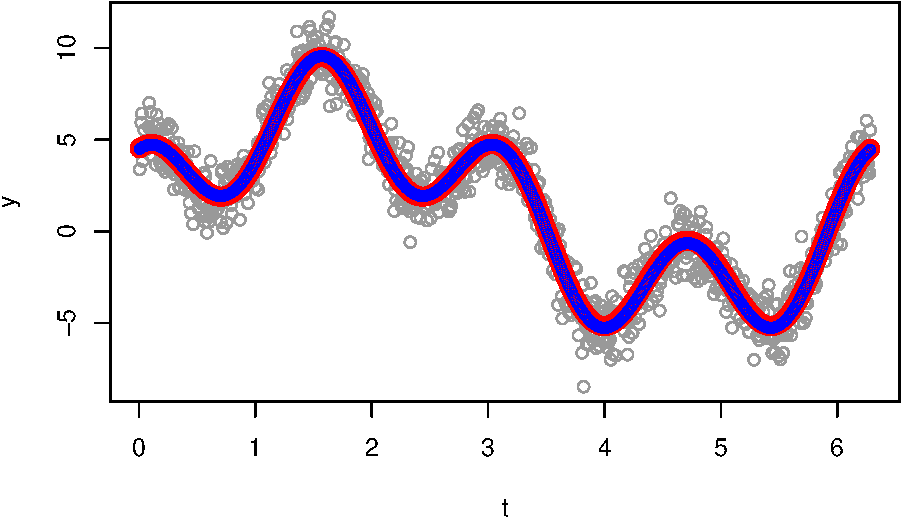
\includegraphics{김남윤_test_1_files/figure-latex/unnamed-chunk-5-1.pdf}
\#\#1-(6)번

\begin{Shaded}
\begin{Highlighting}[]
\NormalTok{X}\OtherTok{\textless{}{-}}\FunctionTok{cbind}\NormalTok{(}\DecValTok{1}\NormalTok{,x1,x2)}
\NormalTok{Y}\OtherTok{\textless{}{-}}\FunctionTok{cbind}\NormalTok{(y)}
\NormalTok{A}\OtherTok{\textless{}{-}} \FunctionTok{t}\NormalTok{(X)}
\NormalTok{B}\OtherTok{\textless{}{-}} \FunctionTok{solve}\NormalTok{(A}\SpecialCharTok{\%*\%}\NormalTok{X)}
\NormalTok{hatβ }\OtherTok{\textless{}{-}}\NormalTok{ B }\SpecialCharTok{\%*\%}\NormalTok{ A }\SpecialCharTok{\%*\%}\NormalTok{ Y}
\end{Highlighting}
\end{Shaded}

\#\#1-(7)번

\begin{Shaded}
\begin{Highlighting}[]
\NormalTok{Xhatβ }\OtherTok{\textless{}{-}}\NormalTok{ X}\SpecialCharTok{\%*\%}\NormalTok{hatβ}
\FunctionTok{plot}\NormalTok{(t,y,}\AttributeTok{col=}\StringTok{\textquotesingle{}gray60\textquotesingle{}}\NormalTok{)}
\FunctionTok{lines}\NormalTok{(t,j,}\AttributeTok{col=}\StringTok{\textquotesingle{}red\textquotesingle{}}\NormalTok{,}\AttributeTok{lwd=}\StringTok{\textquotesingle{}5\textquotesingle{}}\NormalTok{)}
\FunctionTok{lines}\NormalTok{(t,Xhatβ,}\AttributeTok{lty=}\StringTok{"dashed"}\NormalTok{,}\AttributeTok{col=}\StringTok{"blue"}\NormalTok{,}\AttributeTok{lwd=}\StringTok{\textquotesingle{}5\textquotesingle{}}\NormalTok{)}
\end{Highlighting}
\end{Shaded}

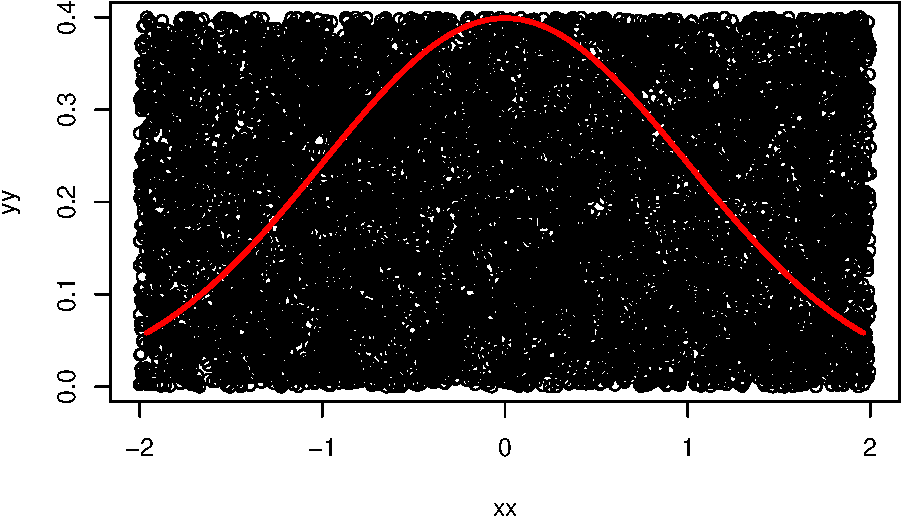
\includegraphics{김남윤_test_1_files/figure-latex/unnamed-chunk-7-1.pdf}
\#\#2-(1)번

\begin{Shaded}
\begin{Highlighting}[]
\NormalTok{x}\OtherTok{=}\FunctionTok{seq}\NormalTok{(}\AttributeTok{from=}\SpecialCharTok{{-}}\FloatTok{1.96}\NormalTok{, }\AttributeTok{to=}\FloatTok{1.96}\NormalTok{ , }\AttributeTok{by=}\FloatTok{0.01}\NormalTok{)}
\NormalTok{y}\OtherTok{=}\DecValTok{1}\SpecialCharTok{/}\FunctionTok{sqrt}\NormalTok{(}\DecValTok{2}\SpecialCharTok{*}\NormalTok{pi)}\SpecialCharTok{*}\FunctionTok{exp}\NormalTok{(}\SpecialCharTok{{-}}\NormalTok{x}\SpecialCharTok{\^{}}\DecValTok{2}\SpecialCharTok{/}\DecValTok{2}\NormalTok{)}
\FunctionTok{plot}\NormalTok{(x,y)}
\end{Highlighting}
\end{Shaded}

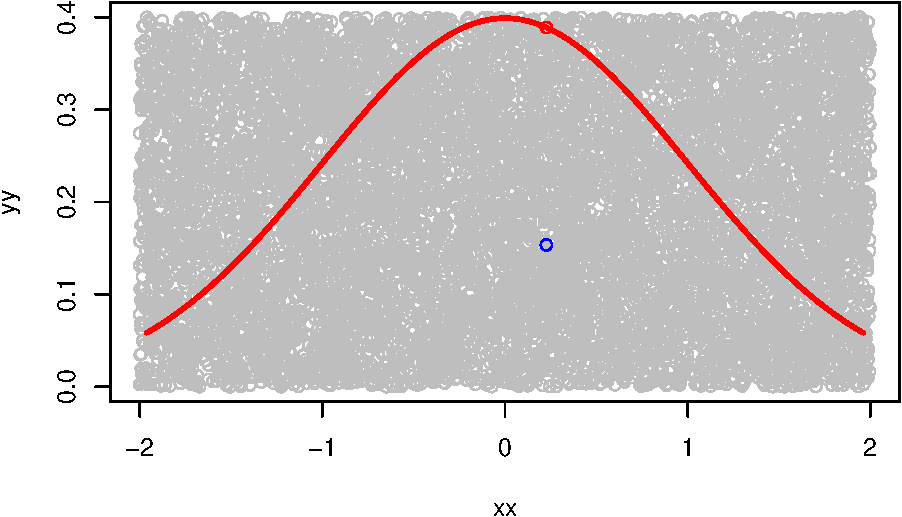
\includegraphics{김남윤_test_1_files/figure-latex/unnamed-chunk-8-1.pdf}

\begin{Shaded}
\begin{Highlighting}[]
\NormalTok{xx}\OtherTok{=}\FunctionTok{runif}\NormalTok{(}\DecValTok{10000}\NormalTok{)}\SpecialCharTok{*}\DecValTok{4{-}2}
\NormalTok{yy}\OtherTok{=}\FunctionTok{runif}\NormalTok{(}\DecValTok{10000}\NormalTok{)}
\FunctionTok{plot}\NormalTok{(xx,yy)}
\FunctionTok{lines}\NormalTok{(x,y,}\AttributeTok{col=}\StringTok{\textquotesingle{}red\textquotesingle{}}\NormalTok{,}\AttributeTok{lwd=}\DecValTok{3}\NormalTok{)}
\end{Highlighting}
\end{Shaded}

\includegraphics{김남윤_test_1_files/figure-latex/unnamed-chunk-8-2.pdf}

\begin{Shaded}
\begin{Highlighting}[]
\NormalTok{test }\OtherTok{=} \ControlFlowTok{function}\NormalTok{(xx,yy)\{}
\NormalTok{    yy }\SpecialCharTok{\textless{}} \DecValTok{1}\SpecialCharTok{/}\FunctionTok{sqrt}\NormalTok{(}\DecValTok{2}\SpecialCharTok{*}\NormalTok{pi)}\SpecialCharTok{*}\FunctionTok{exp}\NormalTok{(}\SpecialCharTok{{-}}\NormalTok{xx}\SpecialCharTok{\^{}}\DecValTok{2}\SpecialCharTok{/}\DecValTok{2}\NormalTok{)}
\NormalTok{    \}}
\NormalTok{tst }\OtherTok{=} \FunctionTok{c}\NormalTok{()}
\ControlFlowTok{for}\NormalTok{ (i }\ControlFlowTok{in} \DecValTok{1}\SpecialCharTok{:}\DecValTok{10000}\NormalTok{) tst[i] }\OtherTok{=} \FunctionTok{test}\NormalTok{(xx[i],yy[i])}
\FunctionTok{plot}\NormalTok{(xx,yy,}\AttributeTok{col=}\StringTok{\textquotesingle{}gray\textquotesingle{}}\NormalTok{)}
\FunctionTok{lines}\NormalTok{(x,y,}\AttributeTok{col=}\StringTok{\textquotesingle{}red\textquotesingle{}}\NormalTok{,}\AttributeTok{lwd=}\DecValTok{3}\NormalTok{)}
\FunctionTok{points}\NormalTok{(xx[tst],yy[tst],}\AttributeTok{col=}\StringTok{\textquotesingle{}red\textquotesingle{}}\NormalTok{)}
\end{Highlighting}
\end{Shaded}

\includegraphics{김남윤_test_1_files/figure-latex/unnamed-chunk-8-3.pdf}

\begin{Shaded}
\begin{Highlighting}[]
\FunctionTok{sum}\NormalTok{(tst)}
\end{Highlighting}
\end{Shaded}

\begin{verbatim}
## [1] 2371
\end{verbatim}

\#\#sum(tst)의 개수/1000*4 가 대략적인 넓이

\#\#2-(2)번

\begin{Shaded}
\begin{Highlighting}[]
\FunctionTok{library}\NormalTok{(tidyverse)}
\end{Highlighting}
\end{Shaded}

\begin{verbatim}
## Warning: package 'tidyverse' was built under R version 4.0.3
\end{verbatim}

\begin{verbatim}
## -- Attaching packages --------------------------------------- tidyverse 1.3.1 --
\end{verbatim}

\begin{verbatim}
## v ggplot2 3.3.5     v purrr   0.3.4
## v tibble  3.1.3     v dplyr   1.0.7
## v tidyr   1.1.3     v stringr 1.4.0
## v readr   1.4.0     v forcats 0.5.1
\end{verbatim}

\begin{verbatim}
## Warning: package 'ggplot2' was built under R version 4.0.5
\end{verbatim}

\begin{verbatim}
## Warning: package 'tibble' was built under R version 4.0.5
\end{verbatim}

\begin{verbatim}
## Warning: package 'tidyr' was built under R version 4.0.3
\end{verbatim}

\begin{verbatim}
## Warning: package 'readr' was built under R version 4.0.5
\end{verbatim}

\begin{verbatim}
## Warning: package 'purrr' was built under R version 4.0.3
\end{verbatim}

\begin{verbatim}
## Warning: package 'dplyr' was built under R version 4.0.5
\end{verbatim}

\begin{verbatim}
## Warning: package 'stringr' was built under R version 4.0.5
\end{verbatim}

\begin{verbatim}
## Warning: package 'forcats' was built under R version 4.0.3
\end{verbatim}

\begin{verbatim}
## -- Conflicts ------------------------------------------ tidyverse_conflicts() --
## x dplyr::filter() masks stats::filter()
## x dplyr::lag()    masks stats::lag()
\end{verbatim}

\begin{Shaded}
\begin{Highlighting}[]
\NormalTok{x}\OtherTok{\textless{}{-}}\FunctionTok{rnorm}\NormalTok{(}\DecValTok{1000}\NormalTok{)}
\FunctionTok{dim}\NormalTok{(x) }\OtherTok{=} \FunctionTok{c}\NormalTok{(}\DecValTok{1000}\NormalTok{,}\DecValTok{1}\NormalTok{)}
\NormalTok{X}\OtherTok{\textless{}{-}}\FunctionTok{as\_tibble}\NormalTok{(x)}
\end{Highlighting}
\end{Shaded}

\begin{verbatim}
## Warning: The `x` argument of `as_tibble.matrix()` must have unique column names if `.name_repair` is omitted as of tibble 2.0.0.
## Using compatibility `.name_repair`.
## This warning is displayed once every 8 hours.
## Call `lifecycle::last_lifecycle_warnings()` to see where this warning was generated.
\end{verbatim}

\begin{Shaded}
\begin{Highlighting}[]
\NormalTok{X }\SpecialCharTok{\%\textgreater{}\%} \FunctionTok{filter}\NormalTok{(V1}\SpecialCharTok{\textgreater{}{-}}\FloatTok{1.96} \SpecialCharTok{\&}\NormalTok{ V1}\SpecialCharTok{\textless{}}\FloatTok{1.96}\NormalTok{)}
\end{Highlighting}
\end{Shaded}

\begin{verbatim}
## # A tibble: 952 x 1
##        V1
##     <dbl>
##  1  0.197
##  2 -1.33 
##  3  0.876
##  4  1.78 
##  5  0.149
##  6 -1.23 
##  7  1.70 
##  8 -0.582
##  9  0.351
## 10  0.629
## # ... with 942 more rows
\end{verbatim}

\hypertarget{uxc0acuxc774uxc5d0-uxc788uxb294-uxd655uxb960uxbcc0uxc218uxc758-uxac1cuxc218uxb294-filteruxc758-uxac1cuxc218uxc774uxb2e4.}{%
\subsection{(-1.96\textasciitilde{} 1.96 사이에 있는 확률변수의 개수는
filter의
개수이다.)}\label{uxc0acuxc774uxc5d0-uxc788uxb294-uxd655uxb960uxbcc0uxc218uxc758-uxac1cuxc218uxb294-filteruxc758-uxac1cuxc218uxc774uxb2e4.}}

\hypertarget{uxbc88-a}{%
\subsection{3번 (A)}\label{uxbc88-a}}

\begin{Shaded}
\begin{Highlighting}[]
\NormalTok{APR}\OtherTok{=}\FunctionTok{c}\NormalTok{(}\StringTok{\textquotesingle{}N1\textquotesingle{}}\NormalTok{,}\StringTok{\textquotesingle{}N2\textquotesingle{}}\NormalTok{,}\StringTok{\textquotesingle{}N3\textquotesingle{}}\NormalTok{,}\StringTok{\textquotesingle{}N4\textquotesingle{}}\NormalTok{,}\StringTok{\textquotesingle{}N5\textquotesingle{}}\NormalTok{,}\StringTok{\textquotesingle{}N6\textquotesingle{}}\NormalTok{,}\StringTok{\textquotesingle{}N7\textquotesingle{}}\NormalTok{,}\StringTok{\textquotesingle{}N8\textquotesingle{}}\NormalTok{,}\StringTok{\textquotesingle{}A\textquotesingle{}}\NormalTok{,}\StringTok{\textquotesingle{}N10\textquotesingle{}}\NormalTok{)}
\NormalTok{SURV}\OtherTok{=}\DecValTok{10}
\NormalTok{PLAYER}\OtherTok{=}\NormalTok{APR[SURV]}
\NormalTok{STAGE}\OtherTok{=}\DecValTok{0}
\NormalTok{PROB}\OtherTok{=}\FloatTok{0.5}
\NormalTok{TOSSRSLT}\OtherTok{=}\ConstantTok{NA}
\FunctionTok{library}\NormalTok{(tidyverse)}
\NormalTok{toss}\OtherTok{=}\ControlFlowTok{function}\NormalTok{(p) }\FunctionTok{rbinom}\NormalTok{(}\AttributeTok{n=}\DecValTok{1}\NormalTok{,}\AttributeTok{size=}\DecValTok{1}\NormalTok{,}\AttributeTok{prob=}\NormalTok{p) }\SpecialCharTok{\%\textgreater{}\%}\NormalTok{ as.logical}

\NormalTok{reset}\OtherTok{=}\ControlFlowTok{function}\NormalTok{()\{}
\NormalTok{  TOSSRSLT}\OtherTok{\textless{}\textless{}{-}}\ConstantTok{NA}
\NormalTok{  SURV}\OtherTok{\textless{}\textless{}{-}} \DecValTok{10}
\NormalTok{  STAGE}\OtherTok{\textless{}\textless{}{-}} \DecValTok{0}
\NormalTok{  PLAYER}\OtherTok{\textless{}\textless{}{-}}\NormalTok{ APR[SURV]}
\NormalTok{\}}

\NormalTok{record}\OtherTok{=}\ControlFlowTok{function}\NormalTok{()\{}
  \FunctionTok{list}\NormalTok{(}\AttributeTok{PRE\_TOSSRSLT=}\NormalTok{TOSSRSLT, }\AttributeTok{SURV=}\NormalTok{SURV, }\AttributeTok{STAGE=}\NormalTok{STAGE, }\AttributeTok{PLAYER=}\NormalTok{PLAYER)}
\NormalTok{\}}

\NormalTok{go}\OtherTok{=} \ControlFlowTok{function}\NormalTok{()\{}
\NormalTok{  PROB}\OtherTok{\textless{}\textless{}{-}} \FloatTok{0.5}\SpecialCharTok{+}\NormalTok{(PLAYER}\SpecialCharTok{==}\StringTok{\textquotesingle{}A\textquotesingle{}}\NormalTok{)}\SpecialCharTok{*}\FloatTok{0.45}
\NormalTok{  TOSSRSLT}\OtherTok{\textless{}\textless{}{-}}\FunctionTok{toss}\NormalTok{(PROB)}
  \ControlFlowTok{if}\NormalTok{ (TOSSRSLT}\SpecialCharTok{==}\ConstantTok{FALSE}\NormalTok{) SURV}\OtherTok{\textless{}\textless{}{-}}\NormalTok{SURV}\DecValTok{{-}1}  
\NormalTok{  STAGE}\OtherTok{\textless{}\textless{}{-}}\NormalTok{STAGE}\SpecialCharTok{+}\DecValTok{1}
\NormalTok{  PLAYER}\OtherTok{\textless{}\textless{}{-}}\NormalTok{APR[SURV]}
\NormalTok{\}}

\NormalTok{gogo}\OtherTok{=}\ControlFlowTok{function}\NormalTok{()\{}
      \ControlFlowTok{for}\NormalTok{(i }\ControlFlowTok{in} \DecValTok{1}\SpecialCharTok{:}\DecValTok{20}\NormalTok{)\{ }
        \FunctionTok{go}\NormalTok{() }
       \ControlFlowTok{if}\NormalTok{ (SURV}\SpecialCharTok{==}\DecValTok{0}\NormalTok{) }\ControlFlowTok{break}
\NormalTok{  \}}
\NormalTok{\}}

\NormalTok{gogo\_history}\OtherTok{=}\ControlFlowTok{function}\NormalTok{() \{}
\NormalTok{  rslt\_}\OtherTok{=}\FunctionTok{as\_tibble}\NormalTok{(}\FunctionTok{record}\NormalTok{())}
  \ControlFlowTok{for}\NormalTok{(i }\ControlFlowTok{in} \DecValTok{1}\SpecialCharTok{:}\DecValTok{20}\NormalTok{)\{}
    \FunctionTok{go}\NormalTok{()}
\NormalTok{    rslt\_}\OtherTok{=}\FunctionTok{rbind}\NormalTok{(rslt\_,}\FunctionTok{as\_tibble}\NormalTok{(}\FunctionTok{record}\NormalTok{()))}
\NormalTok{  \}}
  \FunctionTok{print}\NormalTok{(rslt\_)}
\NormalTok{\}}

\NormalTok{simulate\_once}\OtherTok{=}\ControlFlowTok{function}\NormalTok{()\{}
  \FunctionTok{reset}\NormalTok{()}
  \FunctionTok{gogo}\NormalTok{()}
  \FunctionTok{return}\NormalTok{(}\FunctionTok{record}\NormalTok{()}\SpecialCharTok{$}\NormalTok{SURV)}
\NormalTok{\}}

\NormalTok{simrslt}\OtherTok{=}\FunctionTok{c}\NormalTok{()}
\ControlFlowTok{for}\NormalTok{ (i }\ControlFlowTok{in} \DecValTok{1}\SpecialCharTok{:}\DecValTok{1000}\NormalTok{) simrslt[i]}\OtherTok{=}\FunctionTok{simulate\_once}\NormalTok{()}
\FunctionTok{mean}\NormalTok{(simrslt)}
\end{Highlighting}
\end{Shaded}

\begin{verbatim}
## [1] 5.512
\end{verbatim}

\hypertarget{uxbc88b}{%
\subsection{3번(B)}\label{uxbc88b}}

\begin{Shaded}
\begin{Highlighting}[]
\NormalTok{APR}\OtherTok{=}\FunctionTok{c}\NormalTok{(}\StringTok{\textquotesingle{}N10\textquotesingle{}}\NormalTok{,}\StringTok{\textquotesingle{}A\textquotesingle{}}\NormalTok{,}\StringTok{\textquotesingle{}N8\textquotesingle{}}\NormalTok{,}\StringTok{\textquotesingle{}N7\textquotesingle{}}\NormalTok{,}\StringTok{\textquotesingle{}N6\textquotesingle{}}\NormalTok{,}\StringTok{\textquotesingle{}N5\textquotesingle{}}\NormalTok{,}\StringTok{\textquotesingle{}N4\textquotesingle{}}\NormalTok{,}\StringTok{\textquotesingle{}N3\textquotesingle{}}\NormalTok{,}\StringTok{\textquotesingle{}N2\textquotesingle{}}\NormalTok{,}\StringTok{\textquotesingle{}N1\textquotesingle{}}\NormalTok{)}
\NormalTok{SURV}\OtherTok{=}\DecValTok{10}
\NormalTok{PLAYER}\OtherTok{=}\NormalTok{APR[SURV]}
\NormalTok{STAGE}\OtherTok{=}\DecValTok{0}
\NormalTok{PROB}\OtherTok{=}\FloatTok{0.5}
\NormalTok{TOSSRSLT}\OtherTok{=}\ConstantTok{NA}
\FunctionTok{library}\NormalTok{(tidyverse)}

\NormalTok{toss}\OtherTok{=}\ControlFlowTok{function}\NormalTok{(p) }\FunctionTok{rbinom}\NormalTok{(}\AttributeTok{n=}\DecValTok{1}\NormalTok{,}\AttributeTok{size=}\DecValTok{1}\NormalTok{,}\AttributeTok{prob=}\NormalTok{p) }\SpecialCharTok{\%\textgreater{}\%}\NormalTok{ as.logical}

\NormalTok{reset}\OtherTok{=}\ControlFlowTok{function}\NormalTok{()\{}
\NormalTok{  TOSSRSLT}\OtherTok{\textless{}\textless{}{-}}\ConstantTok{NA}
\NormalTok{  SURV}\OtherTok{\textless{}\textless{}{-}} \DecValTok{10}
\NormalTok{  STAGE}\OtherTok{\textless{}\textless{}{-}} \DecValTok{0}
\NormalTok{  PLAYER}\OtherTok{\textless{}\textless{}{-}}\NormalTok{ APR[SURV]}
\NormalTok{\}}

\NormalTok{record}\OtherTok{=}\ControlFlowTok{function}\NormalTok{()\{}
  \FunctionTok{list}\NormalTok{(}\AttributeTok{PRE\_TOSSRSLT=}\NormalTok{TOSSRSLT, }\AttributeTok{SURV=}\NormalTok{SURV, }\AttributeTok{STAGE=}\NormalTok{STAGE, }\AttributeTok{PLAYER=}\NormalTok{PLAYER)}
\NormalTok{\}}

\NormalTok{go}\OtherTok{=} \ControlFlowTok{function}\NormalTok{()\{}
\NormalTok{  PROB}\OtherTok{\textless{}\textless{}{-}}\FloatTok{0.5}\SpecialCharTok{+}\NormalTok{(PLAYER}\SpecialCharTok{==}\StringTok{\textquotesingle{}A\textquotesingle{}}\NormalTok{)}\SpecialCharTok{*}\FloatTok{0.45}
\NormalTok{  TOSSRSLT}\OtherTok{\textless{}\textless{}{-}}\FunctionTok{toss}\NormalTok{(PROB)}
  \ControlFlowTok{if}\NormalTok{ (TOSSRSLT}\SpecialCharTok{==}\ConstantTok{FALSE}\NormalTok{) SURV}\OtherTok{\textless{}\textless{}{-}}\NormalTok{SURV}\DecValTok{{-}1}
\NormalTok{  STAGE}\OtherTok{\textless{}\textless{}{-}}\NormalTok{STAGE}\SpecialCharTok{+}\DecValTok{1}
\NormalTok{  PLAYER}\OtherTok{\textless{}\textless{}{-}}\NormalTok{APR[SURV]}
\NormalTok{\}}

\NormalTok{gogo}\OtherTok{=}\ControlFlowTok{function}\NormalTok{()\{}
  \ControlFlowTok{for}\NormalTok{(i }\ControlFlowTok{in} \DecValTok{1}\SpecialCharTok{:}\DecValTok{20}\NormalTok{)\{ }
    \FunctionTok{go}\NormalTok{() }
    \ControlFlowTok{if}\NormalTok{ (SURV}\SpecialCharTok{==}\DecValTok{0}\NormalTok{) }\ControlFlowTok{break}
\NormalTok{  \}}
\NormalTok{\}}

\NormalTok{gogo\_history}\OtherTok{=}\ControlFlowTok{function}\NormalTok{() \{}
\NormalTok{  rslt\_}\OtherTok{=}\FunctionTok{as\_tibble}\NormalTok{(}\FunctionTok{record}\NormalTok{())}
  \ControlFlowTok{for}\NormalTok{(i }\ControlFlowTok{in} \DecValTok{1}\SpecialCharTok{:}\DecValTok{20}\NormalTok{)\{}
    \FunctionTok{go}\NormalTok{()}
\NormalTok{    rslt\_}\OtherTok{=}\FunctionTok{rbind}\NormalTok{(rslt\_,}\FunctionTok{as\_tibble}\NormalTok{(}\FunctionTok{record}\NormalTok{()))}
\NormalTok{  \}}
  \FunctionTok{print}\NormalTok{(rslt\_)}
\NormalTok{\}}

\NormalTok{simulate\_once}\OtherTok{=}\ControlFlowTok{function}\NormalTok{()\{}
  \FunctionTok{reset}\NormalTok{()}
  \FunctionTok{gogo}\NormalTok{()}
  \FunctionTok{return}\NormalTok{(}\FunctionTok{record}\NormalTok{()}\SpecialCharTok{$}\NormalTok{SURV)}
\NormalTok{\}}

\NormalTok{simrslt}\OtherTok{=}\FunctionTok{c}\NormalTok{()}
\ControlFlowTok{for}\NormalTok{ (i }\ControlFlowTok{in} \DecValTok{1}\SpecialCharTok{:}\DecValTok{1000}\NormalTok{) simrslt[i]}\OtherTok{=}\FunctionTok{simulate\_once}\NormalTok{()}
\FunctionTok{mean}\NormalTok{(simrslt)}
\end{Highlighting}
\end{Shaded}

\begin{verbatim}
## [1] 1.826
\end{verbatim}

\hypertarget{type-a-uxc5d0uxc11c-uxc0b4uxc544uxb0a8uxc744-uxd655uxb960-uxacc4uxc0b0uxacb0uxacfc}{%
\subsection{TYPE A 에서 살아남을 확률
계산결과}\label{type-a-uxc5d0uxc11c-uxc0b4uxc544uxb0a8uxc744-uxd655uxb960-uxacc4uxc0b0uxacb0uxacfc}}

\hypertarget{type-b-uxc5d0uxc11c-uxc0b4uxc544uxb0a8uxc744-uxd655uxb960-uxacc4uxc0b0uxacb0uxacfc}{%
\subsection{TYPE B 에서 살아남을 확률
계산결과}\label{type-b-uxc5d0uxc11c-uxc0b4uxc544uxb0a8uxc744-uxd655uxb960-uxacc4uxc0b0uxacb0uxacfc}}

\hypertarget{uxb530uxb77cuxc11c-type-auxc5d0uxc11c-uxc0b4uxc544uxb0a8uxc744-uxd655uxb960uxc774-uxb354-uxd06cuxb2e4}{%
\subsection{따라서 TYPE A에서 살아남을 확률이 더
크다}\label{uxb530uxb77cuxc11c-type-auxc5d0uxc11c-uxc0b4uxc544uxb0a8uxc744-uxd655uxb960uxc774-uxb354-uxd06cuxb2e4}}

\hypertarget{uxbc88-4}{%
\subsection{4번}\label{uxbc88-4}}

\begin{Shaded}
\begin{Highlighting}[]
\NormalTok{df}\OtherTok{=}\FunctionTok{read\_csv}\NormalTok{(}\StringTok{\textquotesingle{}https://raw.githubusercontent.com/guebin/2021IR/master/\_notebooks/covid19.csv\textquotesingle{}}\NormalTok{)}
\end{Highlighting}
\end{Shaded}

\begin{verbatim}
## 
## -- Column specification --------------------------------------------------------
## cols(
##   year = col_double(),
##   month = col_double(),
##   day = col_double(),
##   prov = col_character(),
##   cases = col_double()
## )
\end{verbatim}

\begin{Shaded}
\begin{Highlighting}[]
\FunctionTok{head}\NormalTok{(df)}
\end{Highlighting}
\end{Shaded}

\begin{verbatim}
## # A tibble: 6 x 5
##    year month   day prov  cases
##   <dbl> <dbl> <dbl> <chr> <dbl>
## 1  2020     1    20 서울      0
## 2  2020     1    20 부산      0
## 3  2020     1    20 대구      0
## 4  2020     1    20 인천      1
## 5  2020     1    20 광주      0
## 6  2020     1    20 대전      0
\end{verbatim}

\begin{Shaded}
\begin{Highlighting}[]
\NormalTok{df }\OtherTok{=} \FunctionTok{as\_tibble}\NormalTok{(df)}
\NormalTok{df }\SpecialCharTok{\%\textgreater{}\%} \FunctionTok{group\_by}\NormalTok{(year)}
\end{Highlighting}
\end{Shaded}

\begin{verbatim}
## # A tibble: 12,294 x 5
## # Groups:   year [2]
##     year month   day prov  cases
##    <dbl> <dbl> <dbl> <chr> <dbl>
##  1  2020     1    20 서울      0
##  2  2020     1    20 부산      0
##  3  2020     1    20 대구      0
##  4  2020     1    20 인천      1
##  5  2020     1    20 광주      0
##  6  2020     1    20 대전      0
##  7  2020     1    20 울산      0
##  8  2020     1    20 세종      0
##  9  2020     1    20 경기      0
## 10  2020     1    20 강원      0
## # ... with 12,284 more rows
\end{verbatim}

\begin{Shaded}
\begin{Highlighting}[]
\DocumentationTok{\#\# 2020년 확진자 수}
\NormalTok{df }\SpecialCharTok{\%\textgreater{}\%} \FunctionTok{filter}\NormalTok{(year}\SpecialCharTok{==}\DecValTok{2020}\NormalTok{) }\SpecialCharTok{\%\textgreater{}\%}\FunctionTok{summarise}\NormalTok{(}\AttributeTok{sum\_cases=}\FunctionTok{sum}\NormalTok{(cases))}
\end{Highlighting}
\end{Shaded}

\begin{verbatim}
## # A tibble: 1 x 1
##   sum_cases
##       <dbl>
## 1     60726
\end{verbatim}

\begin{Shaded}
\begin{Highlighting}[]
\DocumentationTok{\#\#2021년 확진자 수}
\NormalTok{df }\SpecialCharTok{\%\textgreater{}\%} \FunctionTok{filter}\NormalTok{(year}\SpecialCharTok{==}\DecValTok{2021}\NormalTok{) }\SpecialCharTok{\%\textgreater{}\%}\FunctionTok{summarise}\NormalTok{(}\AttributeTok{sum\_cases=}\FunctionTok{sum}\NormalTok{(cases))}
\end{Highlighting}
\end{Shaded}

\begin{verbatim}
## # A tibble: 1 x 1
##   sum_cases
##       <dbl>
## 1    396886
\end{verbatim}

\begin{Shaded}
\begin{Highlighting}[]
\DocumentationTok{\#\#4{-}(2)번}

\NormalTok{df }\SpecialCharTok{\%\textgreater{}\%} \FunctionTok{filter}\NormalTok{(year}\SpecialCharTok{==}\DecValTok{2020} \SpecialCharTok{\&}\NormalTok{ month}\SpecialCharTok{==}\DecValTok{2} \SpecialCharTok{\&}\NormalTok{ day}\SpecialCharTok{\textless{}=}\DecValTok{15}\NormalTok{) }\SpecialCharTok{\%\textgreater{}\%} \FunctionTok{group\_by}\NormalTok{(prov) }\SpecialCharTok{\%\textgreater{}\%} \FunctionTok{summarise}\NormalTok{(}\AttributeTok{confirm=}\NormalTok{(}\FunctionTok{sum}\NormalTok{(cases)))}
\end{Highlighting}
\end{Shaded}

\begin{verbatim}
## # A tibble: 18 x 2
##    prov  confirm
##    <chr>   <dbl>
##  1 강원        0
##  2 검역        0
##  3 경기        9
##  4 경남        0
##  5 경북        0
##  6 광주        2
##  7 대구        0
##  8 대전        0
##  9 부산        0
## 10 서울        5
## 11 세종        0
## 12 울산        0
## 13 인천        0
## 14 전남        1
## 15 전북        0
## 16 제주        0
## 17 충남        0
## 18 충북        0
\end{verbatim}

\hypertarget{uxb144-2uxc6d4-1uxc77c15uxc77c-uxac00uxc7a5uxb9ceuxc740-uxd655uxc9c4uxc790uxac00-uxbc1cuxacacuxb41c-uxc9c0uxc5eduxc740-uxacbduxae309uxba85}{%
\subsection{2020년 2월 1일\textasciitilde15일 가장많은 확진자가 발견된
지역은
경기(9명)}\label{uxb144-2uxc6d4-1uxc77c15uxc77c-uxac00uxc7a5uxb9ceuxc740-uxd655uxc9c4uxc790uxac00-uxbc1cuxacacuxb41c-uxc9c0uxc5eduxc740-uxacbduxae309uxba85}}

\#\#4-(3)번

\begin{Shaded}
\begin{Highlighting}[]
\NormalTok{df }\SpecialCharTok{\%\textgreater{}\%} \FunctionTok{filter}\NormalTok{(year}\SpecialCharTok{==}\DecValTok{2020} \SpecialCharTok{\&}\NormalTok{ month}\SpecialCharTok{==}\DecValTok{2} \SpecialCharTok{\&}\NormalTok{ day}\SpecialCharTok{\textgreater{}=}\DecValTok{16} \SpecialCharTok{\&}\NormalTok{ day }\SpecialCharTok{\textless{}=} \DecValTok{29}\NormalTok{) }\SpecialCharTok{\%\textgreater{}\%} \FunctionTok{group\_by}\NormalTok{(prov) }\SpecialCharTok{\%\textgreater{}\%} \FunctionTok{summarise}\NormalTok{(}\AttributeTok{confirm=}\NormalTok{(}\FunctionTok{sum}\NormalTok{(cases)))}
\end{Highlighting}
\end{Shaded}

\begin{verbatim}
## # A tibble: 18 x 2
##    prov  confirm
##    <chr>   <dbl>
##  1 강원        7
##  2 검역        0
##  3 경기       65
##  4 경남       59
##  5 경북      472
##  6 광주        7
##  7 대구     2055
##  8 대전       13
##  9 부산       75
## 10 서울       62
## 11 세종        1
## 12 울산       17
## 13 인천        5
## 14 전남        1
## 15 전북        4
## 16 제주        2
## 17 충남       48
## 18 충북       10
\end{verbatim}

\hypertarget{uxb144-2uxc6d4-16uxc77c-29uxc77c-uxae4cuxc9c0-uxac00uxc7a5-uxb9ceuxc740-uxd655uxc9c4uxc790uxac00-uxbc1cuxacacuxb41c-uxc9c0uxc5eduxc740-uxb300uxad6c2055uxba85}{%
\subsection{2020년 2월 16일 \textasciitilde{} 29일 까지 가장 많은
확진자가 발견된 지역은
대구(2055명)}\label{uxb144-2uxc6d4-16uxc77c-29uxc77c-uxae4cuxc9c0-uxac00uxc7a5-uxb9ceuxc740-uxd655uxc9c4uxc790uxac00-uxbc1cuxacacuxb41c-uxc9c0uxc5eduxc740-uxb300uxad6c2055uxba85}}

This is an R Markdown document. Markdown is a simple formatting syntax
for authoring HTML, PDF, and MS Word documents. For more details on
using R Markdown see \url{http://rmarkdown.rstudio.com}.

When you click the \textbf{Knit} button a document will be generated
that includes both content as well as the output of any embedded R code
chunks within the document. You can embed an R code chunk like this:

\begin{Shaded}
\begin{Highlighting}[]
\FunctionTok{summary}\NormalTok{(cars)}
\end{Highlighting}
\end{Shaded}

\begin{verbatim}
##      speed           dist       
##  Min.   : 4.0   Min.   :  2.00  
##  1st Qu.:12.0   1st Qu.: 26.00  
##  Median :15.0   Median : 36.00  
##  Mean   :15.4   Mean   : 42.98  
##  3rd Qu.:19.0   3rd Qu.: 56.00  
##  Max.   :25.0   Max.   :120.00
\end{verbatim}

\hypertarget{including-plots}{%
\subsection{Including Plots}\label{including-plots}}

You can also embed plots, for example:

\includegraphics{김남윤_test_1_files/figure-latex/pressure-1.pdf}

Note that the \texttt{echo\ =\ FALSE} parameter was added to the code
chunk to prevent printing of the R code that generated the plot.

\end{document}
